\documentclass[10pt,a4paper]{article}

\usepackage[scaled]{helvet}
\usepackage[left=2.5cm,right=2.5cm,top=3cm,bottom=3cm]{geometry}
\usepackage{parskip} % don't indent first line of paragraph
\usepackage[utf8x]{inputenc} % e.g. √
\usepackage[none]{hyphenat}\sloppy  % don't hyphenate
\usepackage{tocloft}\addtolength{\cftsubsubsecnumwidth}{0.5em}\tocloftpagestyle{fancy} % fix ToC spacing issue
\usepackage{float} % [H]
\usepackage{fancyref} % \Fref
\usepackage{csquotes} % \nquote
\usepackage{enumitem} % [nolistsep]
\usepackage[printonlyused,withpage]{acronym}
\usepackage{tabularx}
\usepackage{makecell}
\usepackage[table]{xcolor}
\usepackage[hidelinks]{hyperref}\hypersetup{colorlinks, allcolors=., urlcolor=teal}
\usepackage[skins]{tcolorbox}
\usepackage{fancyhdr}
\usepackage{titling} % \thetitle, \theauthor
\usepackage{longtable}
\usepackage{array} % \arraybackslash
\usepackage{multicol}
\usepackage{textcomp} % symbols, e.g. \textdegree
\usepackage{textgreek} % greek letters, e.g. \textmu
\usepackage[super]{nth}
\usepackage{sansmath}\sansmath
\usepackage{amsmath} % bmatrix
\usepackage{svg}
\usepackage{macros} % project specific macros

\renewcommand\familydefault{\sfdefault}

\pagestyle{fancy}
\fancyhf{}
\fancyhead[L]{\thetitle{} \version\\ \thedate}
\fancyfoot[R]{\thepage}
\setlength{\headheight}{29pt} % must be large enough for image
\rhead{\includesvg[width=1.5cm]{Images/xioLogo.svg}}
\renewcommand{\headrulewidth}{0.5pt}
\renewcommand{\footrulewidth}{0.5pt}

\renewcommand\labelitemi{\boldmath$\cdot$} % bullet point
\renewcommand\labelitemii{-} % nested bullet point

\author{x-io Technologies}
\title{x-IMU3 User Manual}
\newcommand{\version}{v1.1}
\date{\today}

\begin{document}
    \begin{center}
    \vglue 5em
    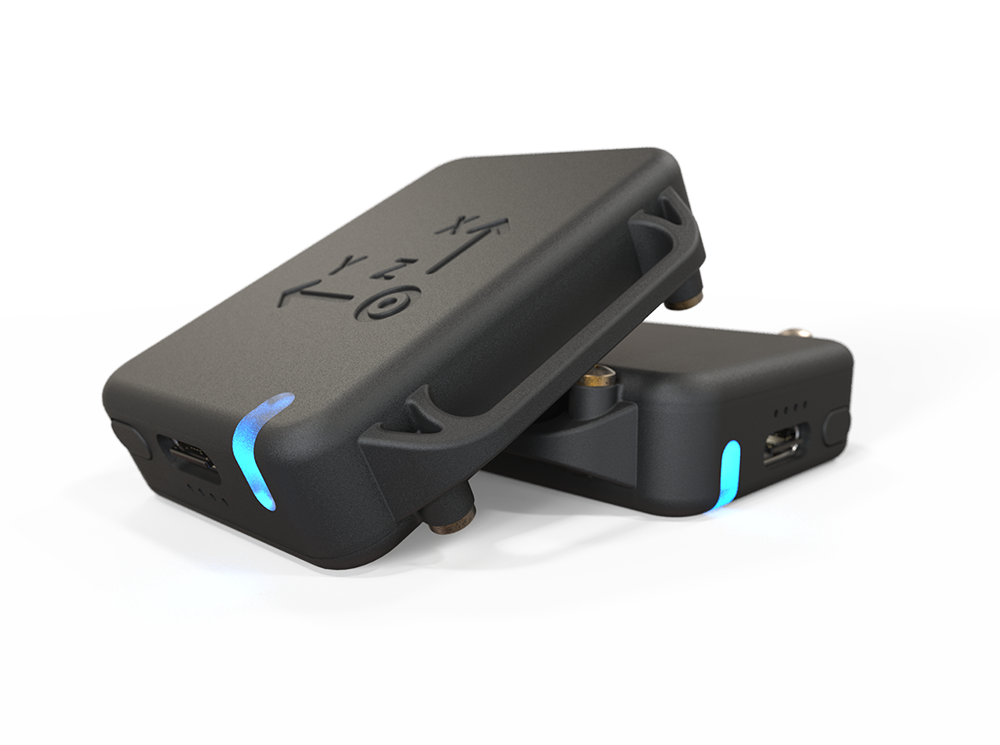
\includegraphics[width=0.8\textwidth]{Images/titlePage.png}
    \vskip 3em
    \Large\textbf{\thetitle}
    \vskip 2em
    \Large{\version}
    \vskip 1em
    \Large{\thedate}
    \vskip 2em
    \large{\theauthor}
\end{center}


    \clearpage
    \tableofcontents

    \clearpage
    \section{Overview}

\begin{multicols}{2}

The x-IMU3 is x-io Technologies' third generation \ac{IMU}.  It is a high-performance and versatile measurement device designed to accommodate a wide range of data logging and real-time applications including biomechanics, motion-capture, virtual reality, drones, robotics, and industrial.

\acs{USB}, Wi-Fi and Bluetooth provide connectivity for mobile and desktop devices while serial communication supports embedded and industrial systems.  An on-board micro \acs{SD} card allows the x-IMU3 to function as a stand-alone data logger with the ability to download files by USB and Wi-Fi.  Multiple x-IMU3s operating together on the same wireless network will automatically synchronise to stream or log synchronised measurements.

\textbf{Sensors}
\begin{itemize}[nolistsep]
    \item Gyroscope, \textpm{}2000\textdegree{}/s, 400 Hz
    \item Accelerometer, \textpm{}24 g, 400 Hz
    \item Magnetometer, \textpm{}2.5 uT, 20 Hz
    \item High-g accelerometer, \textpm{}200 g, 1600 Hz
    \item Temperature sensor\footnote{The temperature sensor is used for calibration and is not intended to provide an accurate measurement of ambient temperature.}
\end{itemize}

\textbf{Calibration}
\begin{itemize}[nolistsep]
    \item 12-parameter calibration for: axis sensitivity, axis bias, inter-axis misalignment, and package misalignment.
    \item Hard-iron and soft-iron calibration
    \item On-board gyroscope bias correction algorithm
\end{itemize}

\textbf{\acs{AHRS}}
\begin{itemize}[nolistsep]
    \item Algorithm outputs:
    \begin{itemize}
        \item Quaternion
        \item Rotation matrix
        \item Euler angles
        \item Linear acceleration
        \item Earth acceleration
    \end{itemize}
    \item Linear acceleration rejection
    \item Magnetic distortion rejection
    \item 400 Hz update rate
    \item Static accuracy:
        \begin{itemize}
            \item 1\textdegree{} \acs{RMS} inclination
            \item 2\textdegree{} \acs{RMS} heading
        \end{itemize}
\end{itemize}

\columnbreak

\textbf{Communication}
\begin{itemize}[nolistsep]
    \item \acs{USB} (\acs{CDC})
    \item Serial, 3.3V \acs{UART}
    \item \acs{TCP} (Wi-Fi)
    \item \acs{UDP} (Wi-Fi)
    \item Bluetooth (\acs{SPP})
\end{itemize}

\textbf{Wi-Fi}
\begin{itemize}[nolistsep]
    \item Client and \acs{AP} mode
    \item Dual band (2.4 GHz, 5 GHz)
    \item WPA/WPA2-Personal
    \item WPA/WPA2-Enterprise\footnote{WPA/WPA2-Enterprise security is only supported in client mode.} (TBC)
\end{itemize}

\textbf{Data logging}
\begin{itemize}[nolistsep]
    \item Supports \acs{SD} cards up to 32 GB\footnote{The product is supplied with an 8 GB \acs{SD} card that can be upgraded by the user.}
    \item Start/stop logging remotely
    \item USB download
    \item Wi-Fi download
    \item \acs{CSV} output
\end{itemize}

\textbf{Serial accessories}
\begin{itemize}[nolistsep]
    \item Receive data from external sensors and user electronics, e.g. \acs{GPS}, analogue/digital inputs, application-specific sensors.
    \item 3.3 V output to power external electronics
\end{itemize}

\textbf{Battery}
\begin{itemize}[nolistsep]
    \item Internal battery charged by \acs{USB}
    \item 15 hours data logging
    \item 11 hours Bluetooth
    \item 9 hours Wi-Fi client 2.4 GHz
    \item 6 hours Wi-Fi client 5 GHz
\end{itemize}

\textbf{Housing}
\begin{itemize}[nolistsep]
    \item IP67 (TBC)
    \item Wearable strap or chassis mount
\end{itemize}

\textbf{Software \acs{GUI}}
\begin{itemize}[nolistsep]
    \item Real-time data plots and 3D view
    \item Log real-time data to \acs{CSV}
    \item Forward real-time data to other applications
    \item Windows and OSX
\end{itemize}

\textbf{Software \acs{API}}
\begin{itemize}[nolistsep]
    \item Rust, C, C++, C\#, Python
    \item Code examples for other languages available
\end{itemize}

\end{multicols}

\clearpage

    \section{Hardware}

\subsection{Board}

Board components are annotated in \Fref{fig:board}.  A detailed mechanical drawing describing the board dimensions and locations of key components is available on the \productWebPage{}.

\vskip 2em

\begin{figure}[H]
    \centering
    \begin{tikzpicture}[annotation/.style={circle, draw=black, fill=white, very thick, minimum size=7mm}]
        \node at (0,0) {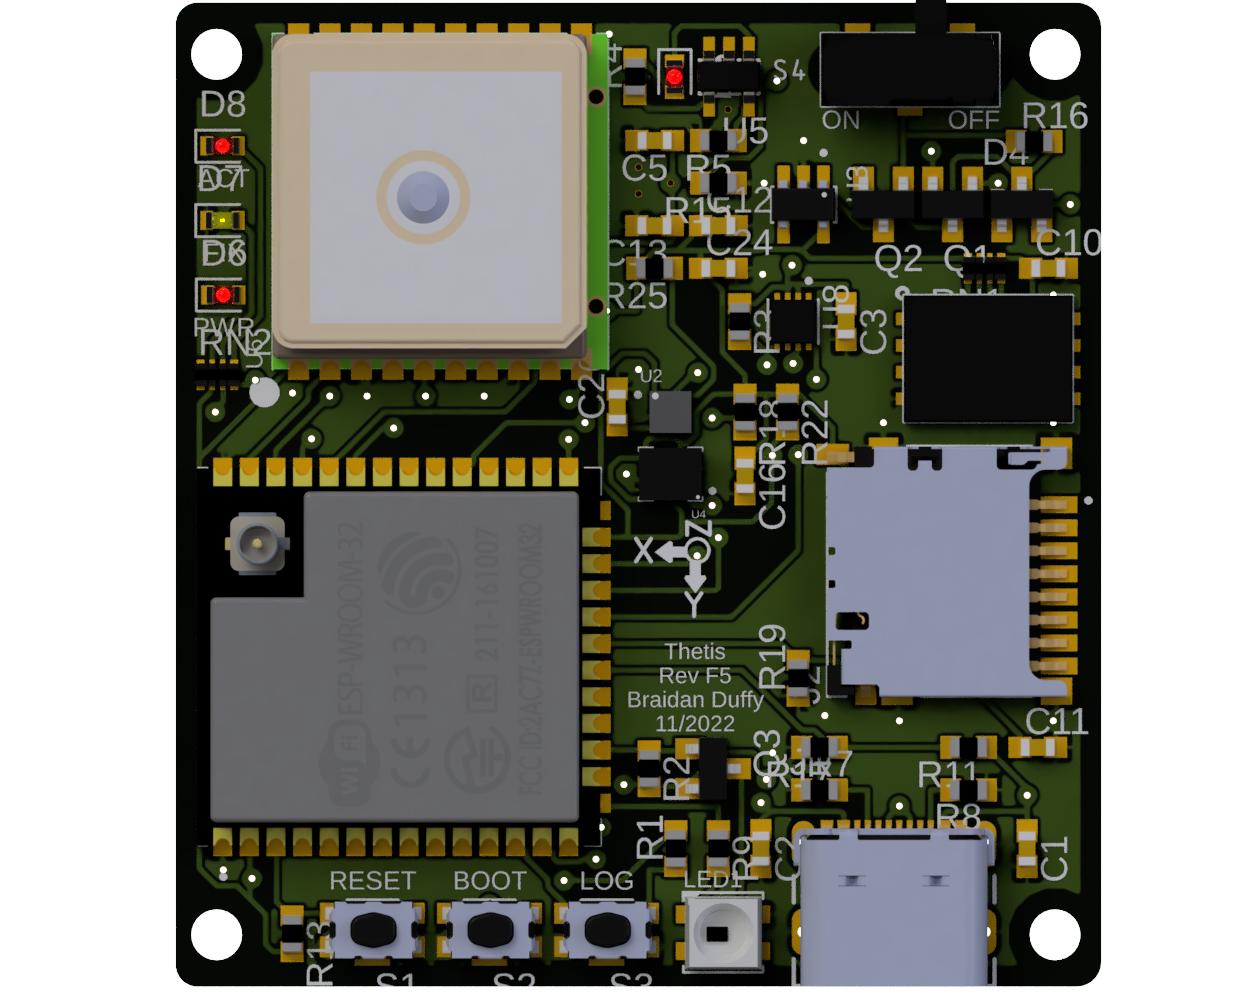
\includegraphics[width=0.95\textwidth]{Images/board.png}};
        \node[annotation] at (-6,-4) {\ref{itm:board1}};
        \node[annotation] at (-6.4,0) {\ref{itm:board2}};
        \node[annotation] at (-5.7,3.7) {\ref{itm:board3}};
        \node[annotation] at (-2.7,1.1) {\ref{itm:board4}};
        \node[annotation] at (4.8,1.8) {\ref{itm:board5}};
        \node[annotation] at (6.0,3.4) {\ref{itm:board6}};
        \node[annotation] at (7.2,3.4) {\ref{itm:board7}};
        \node[annotation] at (6.8,-1.9) {\ref{itm:board8}};
        \node[annotation] at (5.5,-4) {\ref{itm:board9}};
        \node[annotation] at (0.4,-0.8) {\ref{itm:board10}};
        \node[annotation] at (-3.4,-2.9) {\ref{itm:board11}};
    \end{tikzpicture}
    \caption{Board}
    \label{fig:board}
\end{figure}

\vskip 1em

\begin{enumerate}
    \item \label{itm:board1} Power button
    \item \label{itm:board2} \acs{USB}-C connector
    \item \label{itm:board3} \acs{LED}
    \item \label{itm:board4} Serial header
    \item \label{itm:board5} High-g accelerometer
    \item \label{itm:board6} Inertial sensor (gyroscope and accelerometer)
    \item \label{itm:board7} Magnetometer
    \item \label{itm:board8} Wireless antennae
    \item \label{itm:board9} U.FL connector for external wireless antennae
    \item \label{itm:board10} Micro \acs{SD} card socket
    \item \label{itm:board11} Battery connector
\end{enumerate}

\clearpage

\subsection{Housing}

The housing interfaces are annotated in \Fref{fig:housing}.  A detailed mechanical drawing describing the housing dimensions is available on the \productWebPage{}.

\vskip 2em

\begin{figure}[H]
    \centering
    \begin{tikzpicture}[annotation/.style={circle, draw=black, fill=white, very thick, minimum size=7mm}]
        \node at (0,0) {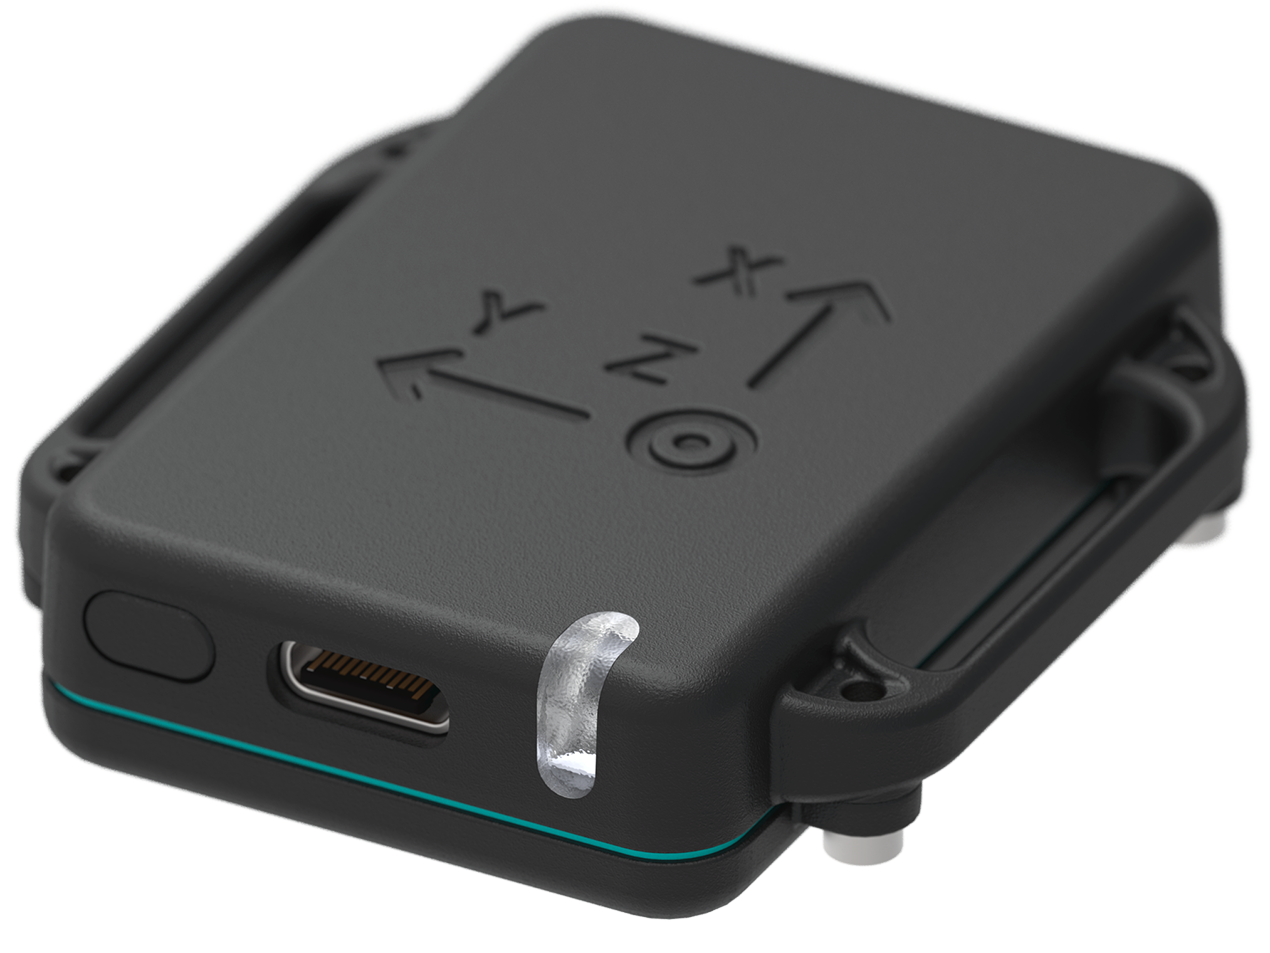
\includegraphics[width=0.8\textwidth]{Images/housing.png}};
        \node[annotation] at (-5.6,-2) {\ref{itm:housing1}};
        \node[annotation] at (-3.7,-2.55) {\ref{itm:housing2}};
        \node[annotation] at (-1.2,-3.2) {\ref{itm:housing3}};
    \end{tikzpicture}
    \caption{Housing}
    \label{fig:housing}
\end{figure}

\vskip 1em

\begin{enumerate}
    \item \label{itm:housing1} Power button
    \item \label{itm:housing2} \acs{USB}-C connector
    \item \label{itm:housing3} \acs{LED}
\end{enumerate}

\subsubsection{\acs{IP67} rating}

The \ac{IP67} rating is an international standard that describes the ability of the housing to protect against the ingress of solid particles and water.  The first digit, 6 indicates complete protection against dust and solid particles.  The second digit, 7 indicates protection from water for a maximum depth of 1 meter for up to 30 minutes.

In practical terms, this means that the housing can be used outdoors in all weather conditions and that it will survive accidental or temporary submersion in water.  The housing should \underline{not} be used in underwater applications.

% The \acs{USB}-C connector is \ac{IP67} rated and does not require a plug to...  However, the connector contains small electrical contacts that can be damaged by dirt or corrosion.  It is recommended that the \acs{USB}-C connector is protected if the housing is expected to be exposed to dust or moisture.

\clearpage

    \section{Technical specification}

\newcommand{\characteristicTable}[4]{
    \customTable
    {l c c}
    {Characteristic & Value & Notes}
    {
        #1
    }
    {#2}
    {#3}
    \textbf{Notes}
    \begin{enumerate}[nolistsep]
        #4
    \end{enumerate}
}

\subsection{Temperature}
\label{sec:temperature}

\newcommand{\noteHeat}{The temperature of the device will always be greater than the surroundings due to heat generated by electronics.}

\newcommand{\noteFullRange}{The specified accuracy of the device is not achieved over the full operating temperature range.  \seeSection{sec:calibration}}

\subsubsection{No battery}

\characteristicTable
{
    Operating & -40\textdegree{}C to 85\textdegree{}C & \ref{itm:temperatureNoBattery1}, \ref{itm:temperatureNoBattery2}\\
    Storage & -40\textdegree{}C to 105\textdegree{}C & -\\
}
{Temperature specification (no battery)}
{tab:temperatureSpecificationNoBattery}
{
    \item \label{itm:temperatureNoBattery1} \noteHeat
    \item \label{itm:temperatureNoBattery2} \noteFullRange
}

\subsubsection{With battery}

\characteristicTable
{
    Operating (discharging) & -20\textdegree{}C to 60\textdegree{}C & \ref{itm:temperatureWithBattery1}, \ref{itm:temperatureWithBattery2}\\
    Operating (charging) & 0\textdegree{}C to 45\textdegree{}C & \ref{itm:temperatureWithBattery1}, \ref{itm:temperatureWithBattery2}, \ref{itm:temperatureWithBattery3}\\
    Storage & -20\textdegree{}C to 25\textdegree{}C & -\\
}
{Temperature specification (with battery)}
{tab:temperatureSpecificationWithBattery}
{
    \item \label{itm:temperatureWithBattery1} \noteHeat
    \item \label{itm:temperatureWithBattery2} \noteFullRange
    \item \label{itm:temperatureWithBattery3} Charging at temperatures below 0\textdegree{}C will reduce the capacity and cycle life of the battery.
}

\subsection{Sensors}

\newcommand{\noteSampleRate}{Each sample includes a timestamp for a reliable measurement of time independent of the sample rate error.  \seeSection{sec:sampleRatesMessageRatesAndTimestamps}}

\newcommand{\noteBandwidth}{The maximum bandwidth is achieved when the message rate is equal to the sample rate.  If the message rate is less than the sample rate then samples are averaged.  \seeSection{sec:sampleRatesMessageRatesAndTimestamps}}

\newcommand{\noteAccuracy}[3]{The accuracy at 1 #1 is evaluated as the deviation of the measured magnitude of #2 for a 360\textdegree{} rotation around the X, Y, and Z axis aligned to the #3 axis.}

\newcommand{\noteTemperature}{Accuracy is specified for the calibrated temperature only.  \seeSection{sec:calibration}}

\subsubsection{Gyroscope}

\characteristicTable
{
    Range & \textpm{}2000\textdegree{}/s & -\\
    Resolution & 16-bit, 0.061\textdegree{}/s & -\\
    Sample rate & 400 Hz \textpm{}0.3\% & \ref{itm:gyroscope1}\\
    Bandwidth & 47 Hz & \ref{itm:gyroscope2}\\
    Noise & 0.014\textdegree{}/s/√Hz & -\\
}
{Gyroscope specification}
{tab:gyroscopeSpecification}
{
    \item \label{itm:gyroscope1} \noteSampleRate
    \item \label{itm:gyroscope2} \noteBandwidth
}

\subsubsection{Accelerometer}

\characteristicTable
{
    Range & \textpm{}24 g & -\\
    Resolution & 16-bit, 732 \textmugreek{}g & -\\
    Sample rate & 400 Hz \textpm{}0.3\% & \ref{itm:accelerometer1}\\
    Bandwidth & 145 Hz & \ref{itm:accelerometer2}\\
    Noise & 160 \textmugreek{}g/√Hz (X, Y), 190 \textmugreek{}g/√Hz (Z) & -\\
    Accuracy at 1 g & TBC & \ref{itm:accelerometer3}, \ref{itm:accelerometer4}\\
}
{Accelerometer specification}
{tab:accelerometerSpecification}
{
    \item \label{itm:accelerometer1} \noteSampleRate
    \item \label{itm:accelerometer2} \noteBandwidth
    \item \label{itm:accelerometer3} \noteAccuracy{g}{gravity}{horizontal}
    \item \label{itm:accelerometer4} \noteTemperature
}

\subsubsection{Magnetometer}

\characteristicTable
{
    Range & \textpm{}1300 \textmugreek{}T (X, Y), \textpm{}2500 \textmugreek{}T (Z) & -\\
    Sample rate & 20 Hz \textpm{}8\% & \ref{itm:magnetometer1}\\
    Noise & 0.3 \textmugreek{}T & -\\
    Accuracy at 1 \acs{a.u.} & TBC & \ref{itm:magnetometer2}, \ref{itm:magnetometer3}, \ref{itm:magnetometer4}\\
}
{Magnetometer specification}
{tab:magnetometerSpecification}
{
    \item \label{itm:magnetometer1} \noteSampleRate
    \item \label{itm:magnetometer2} The calibrated magnetometer units are \ac{a.u.}.  1 \ac{a.u.} is equal to the magnitude of the ambient magnetic field during calibration, approximately 50 \textmugreek{}T.
    \item \label{itm:magnetometer3} \noteAccuracy{\ac{a.u.}}{the ambient magnetic field}{vertical}
    \item \label{itm:magnetometer4} \noteTemperature
}

\subsubsection{High-g accelerometer}

\characteristicTable
{
    Range & \textpm{}200 g & -\\
    Resolution & 16-bit, 6.1 mg & -\\
    Sample rate & 1600 Hz \textpm{}2\% & \ref{itm:highGAccelerometer1}\\
    Bandwidth & 800 Hz & \ref{itm:highGAccelerometer2}\\
    Noise & 5 mg/√Hz & -\\
    Accuracy at 1 g & TBC & \ref{itm:highGAccelerometer3}, \ref{itm:highGAccelerometer4}\\
}
{High-g Accelerometer specification}
{tab:highGAccelerometerSpecification}
{
    \item \label{itm:highGAccelerometer1} \noteSampleRate
    \item \label{itm:highGAccelerometer2} \noteBandwidth
    \item \label{itm:highGAccelerometer3} \noteAccuracy{g}{gravity}{horizontal}
    \item \label{itm:highGAccelerometer4} \noteTemperature
}

\subsubsection{Temperature sensor}

\characteristicTable
{
    Range & -104\textdegree{}C to 150\textdegree{}C & \ref{itm:temperatureSensor1}\\\
    Sample rate & 5 Hz \textpm{}0.3\% & \ref{itm:temperatureSensor2}, \ref{itm:temperatureSensor3}\\
    Accuracy & \textpm{}1\textdegree{}C at 25\textdegree{}C & -\\
}
{Temperature sensor specification}
{tab:temperatureSensor}
{
    \item \label{itm:temperatureSensor1} The temperature sensor measurement range exceeds the device operating temperature range.  \seeSection{sec:temperature}
    \item \label{itm:temperatureSensor2} \noteSampleRate
    \item \label{itm:temperatureSensor3} The temperature sensor is oversampled and the result decimated to the specified sample rate.
}

% \subsection{\acs{AHRS}}

% ...

% \subsection{Latency}

% ...

% \subsection{Wireless throughput}

% ...

% \subsection{Battery life}

% \subsubsection{Data logger}

% ...

% \subsubsection{W-Fi client 2.4 GHz}

% ...

% \subsubsection{W-Fi client 5 GHz}

% ...

% \subsubsection{W-Fi AP 2.4 GHz}

% ...

% \subsubsection{W-Fi AP 5 GHz}

% ...

% \subsection{Example message rates}

% Some aspect of performance is often dependent on message rates.

% % Performance is dependent on send rates... Here are some exmaples
% % - Default message rate
% % - IMU maximum
% % - All maximum

% % binary

% \customTable
% {l c c c}
% {Message type & Default & IMU maximum & All maximum}
% {
%     Inertial (gyroscope and accelerometer) & 50 & 400 & 400\\
%     Magnetometer & 20 & 20 & 20\\
%     AHRS (quaternion) & 50 & 400 & 400\\
%     Temperature & 1 & 1 & 5\\
%     High-g & 50 & 0 & 1600\\
%     Battery & 1 & 1 & 5\\
%     Wi-Fi \acs{RSSI} & 0 & 0 & 1\\
% }
% {Example message rates (messages/s)}
% {tab:exampleMessageRates}

% \subsection{Data logging capacity}

% \Fref{tab:dataLoggingCapacity} summaries the data logging capacity ... continuous logging... for example message rates described in \Fref{tab:exampleMessageRates}.

% \customTable
% {l c c}
% {Message rates & 8 GB & 32 GB}
% {
%     Default & 485 hours & 1941 hours\\
%     IMU maximum & 91 hours & 363 hours\\
%     All maximum & 37 hours & 149 hours\\
% }
% {Data logging capacity}
% {tab:dataLoggingCapacity}

    \section{Calibration}
\label{sec:calibration}

Each device is calibrated during production to achieve the specified accuracy.  The calibration process uses specialist equipment and propriety algorithms to calculate calibration parameters specific to each device.
 Calibration is performed at room temperature.  Accuracy will be reduced for operating temperatures that deviate from this temperature.  Please refer to the calibration certificate for specific temperature values.

\subsection{Inertial sensors}
\label{sec:inertialSensor}

The inertial sensors are the gyroscope, accelerometer, and high-g accelerometer.  Each inertial sensor is calibrated for axis sensitivity, axis offset, inter-axis misalignment, and package misalignment.  The inertial calibration model is described by \Fref{eq:inertial} where $i_c$ is the calibrated inertial measurement obtained from the uncalibrated inertial measurement, $i_u$, given the misalignment matrix, $M$, the sensitivity diagonal matrix, $s$, and the offset vector, $b$.  The inertial calibration model is expanded as \Fref{eq:inertialExpanded} to express the model as 15 scalar quantities.  The units of $i_c$, $i_u$, and $b$ are degrees per second for the gyroscope, and g for the accelerometer and high-g accelerometer.  $M$ and $s$ are ratios and therefore have no units.  The calibration parameters $M$, $s$, and $b$ for each inertial sensor can be accessed as device settings.

\begin{equation}
\label{eq:inertial}
i_c = M s (i_u - b)
\end{equation}

\begin{equation}
\label{eq:inertialExpanded}
    \begin{bmatrix}
        i_{cx}\\
        i_{cy}\\
        i_{cz}\\
    \end{bmatrix}
    =
    \begin{bmatrix}
        m_{xx} & m_{xy} & m_{xz}\\
        m_{yx} & m_{yy} & m_{yz}\\
        m_{zx} & m_{zy} & m_{zz}\\
    \end{bmatrix}
    \begin{bmatrix}
        s_{x} & 0 & 0\\
        0 & s_{y} & 0\\
        0 & 0 & s_{z}\\
    \end{bmatrix}
    \left(
    \begin{bmatrix}
        i_{ux}\\
        i_{uy}\\
        i_{uz}\\
    \end{bmatrix}
    -
    \begin{bmatrix}
        b_{x}\\
        b_{y}\\
        b_{z}\\
    \end{bmatrix}
    \right)
\end{equation}

\subsection{Magnetometer}
\label{sec:magnetometer}

The magnetometer is calibrated for soft iron and hard-iron characteristics.  Soft iron characteristics are distortions that alter the intensity and direction of the magnetic field measured by the magnetometer.  Soft iron calibration also accounts for magnetometer axis sensitivity, inter-axis misalignment, and package misalignment.  Hard iron characteristics are unintended magnetic fields generated by the device that offset magnetometer measurements.  Hard iron calibration also accounts for the magnetometer axis offset.

The magnetometer calibration model is described by \Fref{eq:magnetometer} where $m_c$ is the calibrated magnetometer measurement obtained from the uncalibrated magnetometer measurement, $m_u$, given the soft iron matrix, $S$, the hard iron vector, $h$.  The magnetometer calibration model is expanded as \Fref{eq:magnetometerExpanded} to express the model as 12 scalar quantities.  The units of $m_c$, $m_u$, and $h$ are \ac{a.u.}.  $S$ is a ratio and therefore has no units.  The calibration parameters $S$, $h$ can be accessed as device settings.

\begin{equation}
\label{eq:magnetometer}
m_c = S m_u - h
\end{equation}

\begin{equation}
\label{eq:magnetometerExpanded}
    \begin{bmatrix}
        m_{cx}\\
        m_{cy}\\
        m_{cz}\\
    \end{bmatrix}
    =
    \begin{bmatrix}
        s_{xx} & s_{xy} & s_{xz}\\
        s_{yx} & s_{yy} & s_{yz}\\
        s_{zx} & s_{zy} & s_{zz}\\
    \end{bmatrix}
    \begin{bmatrix}
        m_{ux}\\
        m_{uy}\\
        m_{uz}\\
    \end{bmatrix}
    -
    \begin{bmatrix}
        h_{x}\\
        h_{y}\\
        h_{z}\\
    \end{bmatrix}
\end{equation}

\subsection{Calibration certificate}

Each device is supplied with a calibration certificate.  The calibration certificate details all calibration parameters, the calibration date, the ambient temperature and device temperature during calibration, and any equipment used during the calibration process.  The certificate also includes graphs verifying the accuracy over the measurement range.  Calibration certificates are provided as a \ac{PDF} file.  There are three ways to access the calibration certificate for a device:

\begin{enumerate}[nolistsep]
    \item Scan the \ac{QR} code on the back of the device.
    \item Open the \enquote{Calibration Certificate.html} file stored on the \ac{microSD}.
    \item Enter the device serial number on the calibration certificate \href{https://x-io.co.uk/calibration-certificate/}{web page}.
\end{enumerate}

    \section{Power button}
\label{sec:powerButton}

Pressing the power button while the device is switched off will switch the device on.  The power button must be held for two seconds to switch the device off.  A timestamped notification message containing the string, "Button pressed." is sent each time the button is pressed.  This allows the button to function as a basic user input for real-time applications or as a means marking events during data logging.

    \section{\acs{LED}}
\label{sec:led}

\sectionUnavailable

% ...

% \subsection{Error indication}

% ...

% \subsection{Low battery indication}

% ...

% \subsection{Commands}

% \subsubsection{Strobe}

% ...

% \subsubsection{Colour}

% ...

    \section{Data logger}

The device can function as a stand-alone data logger by streaming real-time data to a file on the micro \ac{SD} card.  Files created by the data logger use the .ximu3 extension and can be downloaded from the device to be converted to \ac{CSV} files using the product software.

The data logger will create a new file in the \enquote{Data Logger} directory on the micro \ac{SD} card each time logging starts.  The data logger will never overwrite data.  If the micro \ac{SD} card becomes full then the data logger will stop and the device will indicate an error.

\subsection{Start and stop}

The data logger is enabled or disabled in the device settings.  If the data logger is enabled then logging will start when the device is switched on and stop when the device is switched off.  Alternatively, an application can start and stop logging remotely by enabling and disabling the data logger while the device is switched on.

Logging will stop automatically when a \ac{USB} host is connected or when a \ac{HTTP} client connects.  The data logger will start again when the \ac{USB} host is disconnected or when the \ac{HTTP} client disconnects.  Connecting \ac{USB} power alone will not stop logging.

\subsection{File name}

The file name format is \enquote{prefix\_YYYY-MM-DD\_hh-mm-ss\_CCCC.ximu3} where where "prefix" is a user-defined label configured in the device settings, \enquote{YYYY-MM-DD\_hh-mm-ss} is the time that the file was created, and \enquote{CCCC} is a counter.  If the prefix is left blank then the device serial number will be used with the format \enquote{XXXX-XXXX-XXXX-XXXX}.  The time and counter parts of the file name can be individually enabled or disabled in the device settings.  For example, if the counter was disabled and the prefix left blank for a device with the serial number \enquote{0123-4567-89AB-CDEF} then a file created at 3.30 p.m. on January 20, 2025 would have the name \enquote{0123-4567-89AB-CDEF\_2025-01-20\_15-30-00.ximu3}.

The counter is a four digit number between 0000 and 9999 that increments each time it is used.  If a file name using the counter already exists then the counter will increment until the file name is available.  Incrementing beyond 9999 will cause the counter to wraparound to 0000.  If the counter part of the file name is disabled and the file name already exists then the counter will used automatically to create an available file name.

\subsection{File contents}

The contents of the file is a byte stream as per the communication protocol described in \Fref{sec:communicationProtocol}.  Each file starts with a preamble of the following messages, in order.

\begin{enumerate}[nolistsep]
    \item Ping response
    \item Write time command
    \item Write setting command for each setting
\end{enumerate}

    \section{Communication protocol}
\label{sec:communicationProtocol}

All communication interfaces use the same communication protocol.  The byte stream is therefore identical for \ac{USB}, serial, \ac{TCP}, \ac{UDP}, and the files created by on-board data logging.  The communication protocol consists of two message types:

\begin{itemize}[nolistsep]
    \item Command messages
    \item Data messages
\end{itemize}

All messages are terminated by a \ac{LF} control character.  This termination byte will not appear anywhere else in a message and so can be used to divide a byte stream into individual messages.  Some messages are terminated with an additional \ac{CR} control character.  \Fref{tab:controlCharactersLFAndCRrepresentations} describes the different ways that the control characters \ac{LF} and \ac{CR} may be referred to throughout this document.

\customTable
{l c c c c}
{Control character & Abbreviation & String & Hex & Decimal}
{
    \acl{LF} & \acs{LF} & \enquote{\textbackslash n} & 0x0A & 10\\
    \acl{CR} & \acs{CR} & \enquote{\textbackslash r} & 0x0D & 13\\
}
{Control characters \acs{LF} and \acs{CR} representations}
{tab:controlCharactersLFAndCRrepresentations}

The first byte of a message indicates the message type.  Command messages start with the character \enquote{\{} (0x7B in hex, 123 in decimal).  Data messages start with either an uppercase character or a byte value greater than 0x80 (128 in decimal) depending on the message.

\subsection{Command messages}

Command messages are sent to the device to read and write settings and execute commands.  All command messages are a \ac{JSON} object containing a single key/value pair, terminated by the control character sequence: \ac{CR}, \ac{LF}.  The control character \ac{LF} must not appear anywhere else in a command message.  The device will acknowledge each received command message by sending a command message with the same key to the host.

The key used by command messages sent to the device is not case sensitive and can use non-alphanumeric characters arbitrarily.  For example, \enquote{serialNumber}, \enquote{Serial Number}, and \enquote{serial\_number} are all valid keys for a command message to read the device serial number.  The key used by the acknowledgement command message sent from the device to the host will always be in camel case. For example, \enquote{serialNumber}.

\subsubsection{Read setting command}

The read setting command is sent to the device to read a setting value.  The key is the setting key and the value is null.  See \Fref{sec:individualSettings} for a complete list of settings.  The device will acknowledge a read setting command by sending a write setting command to the host.

\commandMessageExample{"serialNumber":null}

\subsubsection{Write setting command}

The write setting command is sent to the device to write a setting value.  The key is the setting key and the value is the setting value.  See \Fref{sec:individualSettings} for a complete list of settings.  The device will acknowledge a write setting command by sending a setting write command back to the host, indicating the new settings value.  The device will not apply new settings until two seconds after the most recent write setting command or default command was received.

\commandMessageExample{"deviceName":"x-IMU3"}

\subsubsection{Default command}

The default command is sent to the device to set all settings to default values.  The key is \enquote{default} and the value is null.  The device will not apply new settings until two seconds after the most recent write setting command or default command was received.

\commandMessageExample{"default":null}

\subsubsection{Apply command}

The apply command is sent to the device to apply all settings.  The key is \enquote{apply} and the value is null.  This command can be sent after a write setting or default command to apply settings immediately instead of after a two second delay.

\commandMessageExample{"apply":null}

\subsubsection{Save command}

The save command is sent to the device to save all settings to \ac{NVM}.  The key is \enquote{save} and the value is null.  This command is unnecessary in most applications because the device will automatically save all settings on shutdown.
% This command can be used to ensure settings are saved in applications that remove power from the device instead of performing a shutdown.

\commandMessageExample{"save":null}

\subsubsection{Read time command}

The read time command is sent to the device to read the date and time of the \ac{RTC}.  The key is \enquote{time} and the value is null.  The device will acknowledge a read time command by sending a write time command to the host.

\commandMessageExample{"time":null}

\subsubsection{Write time command}

The write time command is sent to the device to write the date and time of the \ac{RTC}.  The key is \enquote{time} and the value is a string expressing the date and time in the format \enquote{YYYY-MM-DD hh:mm:ss} where each delimiter can be any non-numerical character.  The device will acknowledge a write time command by sending a write time command back to the host, indicating the new date and time.

\commandMessageExample{"time":"2020-01-01 00:00:00"}

\subsubsection{Ping command}

The ping command is sent to the device to trigger a ping response.  The key is \enquote{ping} and the value is null.  The device will acknowledge a ping command by sending a ping response to the host.

\commandMessageExample{"ping":null}

\subsubsection{Ping response}

The ping response is sent from the device to the host in response to the ping command.  The key is \enquote{ping} and the value is a \ac{JSON} object containing three key/value pairs indicating the communication interface, device name, and device serial number.  The keys are \enquote{interface}, \enquote{deviceName}, and \enquote{serialNumber}, respectively and all values are string types.

\begin{table}[H]
    \begin{tabular}{l l l}
        \textbf{Example}*\textbf{:} & \texttt{\{} \\
        & \texttt{~~"ping":~\{} & \\
        & \texttt{~~~~"interface":} & \texttt{"USB",} \\
        & \texttt{~~~~"deviceName":} & \texttt{"x-IMU3",} \\
        & \texttt{~~~~"serialNumber":} & \texttt{"0123-4567-89AB-CDEF"} \\
        & \texttt{~~\}} \\
        & \texttt{\}\textbackslash r\textbackslash n} \\
    \end{tabular} \\
    \begin{tabular}{l}
        \\
        \footnotesize{* The actual \acs{JSON} will not include any whitespace.}
    \end{tabular}
\end{table}

\subsubsection{Reset command}
\label{sec:resetCommand}

The reset command is sent to the device to reset the device.  The key is \enquote{reset} and the value is null.  A reset is equivalent to switching the device off and then on again.  The device will reset two seconds after receiving this command.

\commandMessageExample{"reset":null}

\subsubsection{Shutdown command}
\label{sec:shutdownCommand}

The shutdown command is sent to the device to switch the device off.  The key is \enquote{shutdown} and the value is null.  The device will shutdown two seconds after receiving this command.

\commandMessageExample{"shutdown":null}

% \subsubsection{Set heading command}

% ...

% \commandMessageExample{"heading":0}

\subsubsection{Strobe command}

The strobe command is sent to the device to strobe the \ac{LED} bright white for 5 seconds.  The key is \enquote{strobe} and the value is null.

\commandMessageExample{"strobe":null}

% \subsubsection{Colour command}

% The colour command is sent to the device to set the \ac{LED} colour.  The key is \enquote{colour} or \enquote{color} and the value is either null or an \ac{RGB} hex triplet expressed as a string.
% %
% If the value is an \ac{RGB} hex triplet then the LED will immediately change to the specified colour.  This action overrides the normal LED behaviour and the LED will no longer provide an indication of the device mode or status.
% %
% If the value is null then the LED will revert to its normal behaviour.
% %
% The \enquote{\#} character is optional.  For example, \enquote{\#FF0000} for red or \enquote{\#00FFFF} for cyan.

% % {"colour":[255 255 255]}\n
% % {"strobe":[255 255 255]}\n

% \commandMessageExample{"colour":"\#FFFFFFFF"}

\subsubsection{Serial accessory command}

The serial accessory command is sent to the device to transmit data to a serial accessory when the serial interface is in serial accessory mode.  The key is \enquote{serial} and the value is the data expressed as a string of up to 256 characters.  Longer strings will be truncated to the maximum size.  The string escape sequence \enquote{\textbackslash u} can be used to express any byte value as per the \ac{JSON} specification.

\commandMessageExample{"serial":"hello \textbackslash u0077\textbackslash u006F\textbackslash u0072\textbackslash u006C\textbackslash u0064"}

\subsubsection{Note command}

The note command is sent to the device to generate a timestamped notification message containing a user-defined string.  The key is \enquote{note} and the value is the string of up to 127 characters.  Longer strings will be truncated to the maximum size.  This command can be used to create timestamped notes of events during data logging.

\commandMessageExample{"note":"Something happened."}

\subsubsection{Bootloader command}

The bootloader command is sent to the device to put the device in bootloader mode.  The key is \enquote{bootloader} and the value is null.  The device will enter bootloader mode two seconds after receiving this command.  See \Fref{sec:updatingDeviceFirmware} for more information about updating the device firmware.

\commandMessageExample{"bootloader":null}

\subsection{Data messages}
\label{sec:dataMessages}

Data messages are sent from the device to the host to provide timestamped measurements, serial accessory data, notifications, and error messages.  Data messages will be either \ac{ASCII} or binary, depending on the device settings.

\ac{ASCII} data messages consist of multiple comma-separated values terminated by the control character sequence: \ac{CR}, \ac{LF}.  The first value is a single uppercase character indicating the message type.  The second value is the timestamp in microseconds.  The remaining values are arguments specific to the message type.

Binary data messages are a sequence of bytes terminated by the control character \ac{LF}.  The first byte of the sequence indicates the message type.  The value of this byte is equal to 0x80 plus the first character of the equivalent \ac{ASCII} message.  The next eight bytes are the timestamp in microseconds expressed as a 64-bit unsigned integer.  The remaining bytes are arguments specific to the message type.  Numerical types use little-endian ordering.  Byte stuffing is used to remove all occurrences of the control character \ac{LF} prior to the termination byte.

\subsubsection{Byte stuffing}
\label{sec:byteStuffing}

Byte stuffing ensures that the termination byte value, 0x0A, only occurs at the end of a binary data message.  This is achieved by replacing all occurrences of the termination byte prior to termination with an escape sequence.  This process is identical to \ac{SLIP} except that the \enquote{END} byte value is defined as 0x0A.  \Fref{tab:valuesUsedByTheByteStuffingProcess} lists the values used by the byte stuffing process.

\customTable
{l l l l}
{Hex & Decimal & Name & Description}
{
0x0A & 10 & END & Message termination \\
0xDB & 219 & ESC & Message escape \\
0xDC & 220 & ESC\_END & Transposed message termination \\
0xDD & 221 & ESC\_ESC & Transposed message escape \\
}
{Values used by the byte stuffing process}
{tab:valuesUsedByTheByteStuffingProcess}

Byte stuffing is achieved by the following:

\begin{itemize}
    \item Replace each occurrence of END in the original message with the two byte sequence: ESC, ESC\_END.
    \item Replace each occurrence of ESC in the original message with the two byte sequence: ESC, ESC\_ESC.
\end{itemize}

The byte stuffing process will not modify the END that terminates the message.  \Fref{tab:byteStuffingExamples} demonstrates byte stuffing for example byte sequences terminated as binary data messages.

\begingroup
    \definecolor{colourA}{HTML}{1F77B4} % Tableau colours
    \definecolor{colourB}{HTML}{FF7F0E}
    \definecolor{colourC}{HTML}{2CA02C}
    \customTable
    {c l l}
    {Example & Before byte stuffing & After byte stuffing}
    {
    1 & \texttt{45 58 41 4D 50 4C 45 \textcolor{colourC}{0A}} & \texttt{45 58 41 4D 50 4C 45 \textcolor{colourC}{0A}} \\
    2 & \texttt{45 \textcolor{colourA}{0A} 41 4D 50 4C 45 \textcolor{colourC}{0A}} & \texttt{45 \textcolor{colourA}{DB DC} 41 4D 50 4C 45 \textcolor{colourC}{0A}} \\
    3 & \texttt{45 58 \textcolor{colourB}{DB} 4D 50 4C 45 \textcolor{colourC}{0A}} & \texttt{45 58 \textcolor{colourB}{DB DD} 4D 50 4C 45 \textcolor{colourC}{0A}} \\
    4 & \texttt{45 58 41 4D 50 \textcolor{colourB}{DB} \textcolor{colourA}{0A} \textcolor{colourC}{0A}} & \texttt{45 58 41 4D 50 \textcolor{colourB}{DB DD} \textcolor{colourA}{DB DC} \textcolor{colourC}{0A}} \\
    }
    {Byte stuffing examples}
    {tab:byteStuffingExamples}
\endgroup

\subsubsection{Inertial message}

The inertial message provides timestamped gyroscope and accelerometer measurements.  Inertial messages are sent continuously at the message rate configured in the device settings.  The first value of an \ac{ASCII} message is the character \enquote{I} and the arguments are six numerical values expressed to four decimal places.  The first byte of a binary message is C9 (equal to 0x80 + \enquote{I}) and the arguments are six contiguous 32-bit floats.  The message arguments are described in \Fref{tab:inertialMessageArguments}.

\begingroup
    \def\tempArgumentA{Gyroscope X axis in degrees per second}
    \def\tempArgumentB{Gyroscope Y axis in degrees per second}
    \def\tempArgumentC{Gyroscope Z axis in degrees per second}
    \def\tempArgumentD{Accelerometer X axis in g}
    \def\tempArgumentE{Accelerometer Y axis in g}
    \def\tempArgumentF{Accelerometer Z axis in g}
    \dataMessageTable
    {Inertial message arguments}
    {tab:inertialMessageArguments}
\endgroup

\begingroup
    \def\tempNameA{Gyroscope X axis}
    \def\tempNameB{Gyroscope Y axis}
    \def\tempNameC{Gyroscope Z axis}
    \def\tempNameD{Accelerometer X axis}
    \def\tempNameE{Accelerometer Y axis}
    \def\tempNameF{Accelerometer Z axis}
    \def\tempValueA{0}
    \def\tempValueB{0}
    \def\tempValueC{0}
    \def\tempValueD{0}
    \def\tempValueE{0}
    \def\tempValueF{1}
    \def\tempAsciiFirst{I}
    \def\tempAsciiA{0.0000}
    \def\tempAsciiB{0.0000}
    \def\tempAsciiC{0.0000}
    \def\tempAsciiD{0.0000}
    \def\tempAsciiE{0.0000}
    \def\tempAsciiF{1.0000}
    \def\tempBinaryFirst{C9}
    \def\tempBinaryA{00 00 00 00}
    \def\tempBinaryB{00 00 00 00}
    \def\tempBinaryC{00 00 00 00}
    \def\tempBinaryD{00 00 00 00}
    \def\tempBinaryE{00 00 00 00}
    \def\tempBinaryF{00 00 80 3F}
    \dataMessageExample
\endgroup

\subsubsection{Magnetometer message}

The magnetometer message provides timestamped magnetometer measurements.  Magnetometer messages are sent continuously at the message rate configured in the device settings.  The first value of an \ac{ASCII} message is the character \enquote{M} and the arguments are three numerical values expressed to four decimal places.  The first byte of a binary message is CD (equal to 0x80 + \enquote{M}) and the arguments are three contiguous 32-bit floats.  The message arguments are described in \Fref{tab:magnetometerMessageArguments}.

\begingroup
    \def\tempArgumentA{Magnetometer X axis in arbitrary units}
    \def\tempArgumentB{Magnetometer Y axis in arbitrary units}
    \def\tempArgumentC{Magnetometer Z axis in arbitrary units}
    \dataMessageTable
    {Magnetometer message arguments}
    {tab:magnetometerMessageArguments}
\endgroup

\begingroup
    \def\tempNameA{Magnetometer X axis}
    \def\tempNameB{Magnetometer Y axis}
    \def\tempNameC{Magnetometer Z axis}
    \def\tempValueA{1.0}
    \def\tempValueB{0.0}
    \def\tempValueC{0.0}
    \def\tempAsciiFirst{M}
    \def\tempAsciiA{1.0000}
    \def\tempAsciiB{0.0000}
    \def\tempAsciiC{0.0000}
    \def\tempBinaryFirst{CD}
    \def\tempBinaryA{00 00 80 3F}
    \def\tempBinaryB{00 00 00 00}
    \def\tempBinaryC{00 00 00 00}
    \dataMessageExample
\endgroup

\subsubsection{Quaternion message}

The quaternion message provides timestamped measurement of orientation of the device relative to the Earth.  Quaternion messages are sent continuously at the message rate configured in the device settings.  The first value of an \ac{ASCII} message is the character \enquote{Q} and the arguments are four numerical values expressed to four decimal places.  The first byte of a binary message is D1 (equal to 0x80 + \enquote{Q}) and the arguments are four contiguous 32-bit floats.  The message arguments are described in \Fref{tab:quaternionMessageArguments}.

\begingroup
    \def\tempArgumentA{Quaternion W element}
    \def\tempArgumentB{Quaternion X element}
    \def\tempArgumentC{Quaternion Y element}
    \def\tempArgumentD{Quaternion Z element}
    \def\tempCaption{Quaternion message arguments}
    \def\tempLabel{tab:quaternionMessageArguments}
    \dataMessageTable
    {Quaternion message arguments}
    {tab:quaternionMessageArguments}
\endgroup

\begingroup
    \def\tempNameA{Quaternion W element}
    \def\tempNameB{Quaternion X element}
    \def\tempNameC{Quaternion Y element}
    \def\tempNameD{Quaternion Z element}
    \def\tempValueA{1}
    \def\tempValueB{0}
    \def\tempValueC{0}
    \def\tempValueD{0}
    \def\tempAsciiFirst{Q}
    \def\tempAsciiA{1.0000}
    \def\tempAsciiB{0.0000}
    \def\tempAsciiC{0.0000}
    \def\tempAsciiD{0.0000}
    \def\tempBinaryFirst{D1}
    \def\tempBinaryA{00 00 80 3F}
    \def\tempBinaryB{00 00 00 00}
    \def\tempBinaryC{00 00 00 00}
    \def\tempBinaryD{00 00 00 00}
    \dataMessageExample
\endgroup

\subsubsection{Rotation matrix message}

The rotation matrix message provides timestamped measurement of orientation of the device relative to the Earth.  Rotation matrix messages are sent continuously at the message rate configured in the device settings.  The first value of an \ac{ASCII} message is the character \enquote{R} and the arguments are nine numerical values expressed to four decimal places.  The first byte of a binary message is D2 (equal to 0x80 + \enquote{R}) and the arguments are nine contiguous 32-bit floats.  The message arguments are described in \Fref{tab:rotationMatrixMessageArguments}.

\begingroup
    \def\tempArgumentA{Rotation matrix XX element}
    \def\tempArgumentB{Rotation matrix XY element}
    \def\tempArgumentC{Rotation matrix XZ element}
    \def\tempArgumentD{Rotation matrix YX element}
    \def\tempArgumentE{Rotation matrix YY element}
    \def\tempArgumentF{Rotation matrix YZ element}
    \def\tempArgumentG{Rotation matrix ZX element}
    \def\tempArgumentH{Rotation matrix ZY element}
    \def\tempArgumentI{Rotation matrix ZZ element}
    \dataMessageTable
    {Rotation matrix message arguments}
    {tab:rotationMatrixMessageArguments}
\endgroup

\begingroup
    \def\tempNameA{Rotation matrix XX element}
    \def\tempNameB{Rotation matrix XY element}
    \def\tempNameC{Rotation matrix XZ element}
    \def\tempNameD{Rotation matrix YX element}
    \def\tempNameE{Rotation matrix YY element}
    \def\tempNameF{Rotation matrix YZ element}
    \def\tempNameG{Rotation matrix ZX element}
    \def\tempNameH{Rotation matrix ZY element}
    \def\tempNameI{Rotation matrix ZZ element}
    \def\tempValueA{1}
    \def\tempValueB{0}
    \def\tempValueC{0}
    \def\tempValueD{0}
    \def\tempValueE{1}
    \def\tempValueF{0}
    \def\tempValueG{0}
    \def\tempValueH{0}
    \def\tempValueI{1}
    \def\tempAsciiFirst{R}
    \def\tempAsciiA{1.0000}
    \def\tempAsciiB{0.0000}
    \def\tempAsciiC{0.0000}
    \def\tempAsciiD{0.0000}
    \def\tempAsciiE{1.0000}
    \def\tempAsciiF{0.0000}
    \def\tempAsciiG{0.0000}
    \def\tempAsciiH{0.0000}
    \def\tempAsciiI{1.\linebreak0000} % \texttt will not line break
    \def\tempBinaryFirst{D2}
    \def\tempBinaryA{00 00 80 3F}
    \def\tempBinaryB{00 00 00 00}
    \def\tempBinaryC{00 00 00 00}
    \def\tempBinaryD{00 00 00 00}
    \def\tempBinaryE{00 00 80 3F}
    \def\tempBinaryF{00 00 00 00}
    \def\tempBinaryG{00 00 00 00}
    \def\tempBinaryH{00 00 00 00}
    \def\tempBinaryI{00 00 80 3F}
    \dataMessageExample
\endgroup

\subsubsection{Euler angles message}

The Euler angles message provides timestamped measurement of orientation of the device relative to the Earth.  Euler angles messages are sent continuously at the message rate configured in the device settings.  The first value of an \ac{ASCII} message is the character \enquote{E} and the arguments are three numerical values expressed to four decimal places.  The first byte of a binary message is C5 (equal to 0x80 + \enquote{E}) and the arguments are three contiguous 32-bit floats.  The message arguments are described in \Fref{tab:eulerAnglesMessageArguments}.

\begingroup
    \def\tempArgumentA{Roll angle in degrees}
    \def\tempArgumentB{Pitch angle in degrees}
    \def\tempArgumentC{Yaw angle in degrees}
    \dataMessageTable
    {Euler angles message arguments}
    {tab:eulerAnglesMessageArguments}
\endgroup

\begingroup
    \def\tempNameA{Roll angle}
    \def\tempNameB{Pitch angle}
    \def\tempNameC{Yaw angle}
    \def\tempValueA{0.0}
    \def\tempValueB{0.0}
    \def\tempValueC{0.0}
    \def\tempAsciiFirst{E}
    \def\tempAsciiA{0.0000}
    \def\tempAsciiB{0.0000}
    \def\tempAsciiC{0.0000}
    \def\tempBinaryFirst{C5}
    \def\tempBinaryA{00 00 00 00}
    \def\tempBinaryB{00 00 00 00}
    \def\tempBinaryC{00 00 00 00}
    \dataMessageExample
\endgroup

\subsubsection{Pressure message}

The pressure message provides timestamped barometric pressure and altitude measurements.  Pressure messages are sent continuously at the message rate configured in the device settings.  The first value of an \ac{ASCII} message is the character \enquote{P} and the arguments are two numerical values expressed to four decimal places.  The first byte of a binary message is D0 (equal to 0x80 + \enquote{P}) and the arguments are two contiguous 32-bit floats.  The message arguments are described in \Fref{tab:pressureMessageArguments}.

\begingroup
    \def\tempArgumentA{Barometric air pressure in millibars}
    \def\tempArgumentB{Altitude in metres}
    \dataMessageTable
    {Pressure message arguments}
    {tab:pressureMessageArguments}
\endgroup

\begingroup
    \def\tempNameA{Pressure}
    \def\tempNameB{Altitude}
    \def\tempValueA{1023.14}
    \def\tempValueB{0.0}
    \def\tempAsciiFirst{P}
    \def\tempAsciiA{1023.1400}
    \def\tempAsciiB{0.0000}
    \def\tempBinaryFirst{D0}
    \def\tempBinaryA{00 50 7D 44}
    \def\tempBinaryB{00 00 00 00}
    \dataMessageExample
\endgroup

\subsubsection{Temperature message}

The temperature message provides timestamped temperature measurements.  Temperature messages are sent continuously at the message rate configured in the device settings.  The first value of an \ac{ASCII} message is the character \enquote{T} and the argument is a numerical value expressed to four decimal places.  The first byte of a binary message is D4 (equal to 0x80 + \enquote{T}) and the argument is a 32-bit float.  The message arguments are described in \Fref{tab:temperatureMessageArguments}.

\begingroup
    \def\tempArgumentA{Temperature in degrees Celsius}
    \dataMessageTable
    {Temperature message arguments}
    {tab:temperatureMessageArguments}
\endgroup

\begingroup
    \def\tempNameA{Temperature}
    \def\tempValueA{25}
    \def\tempAsciiFirst{T}
    \def\tempAsciiA{25.0000}
    \def\tempBinaryFirst{D4}
    \def\tempBinaryA{00 00 41 C8}
    \dataMessageExample
\endgroup

\subsubsection{High-g message}

The High-g message provides timestamped high-g accelerometer measurements.  High-g messages are sent continuously at the message rate configured in the device settings.  The first value of an \ac{ASCII} message is the character \enquote{H} and the arguments are three numerical values expressed to four decimal places.  The first byte of a binary message is C8 (equal to 0x80 + \enquote{H}) and the arguments are three contiguous 32-bit floats.  The message arguments are described in \Fref{tab:highGMessageArguments}.

\begingroup
    \def\tempArgumentA{High-g accelerometer X axis in g}
    \def\tempArgumentB{High-g accelerometer Y axis in g}
    \def\tempArgumentC{High-g accelerometer Z axis in g}
    \dataMessageTable
    {High-g message arguments}
    {tab:highGMessageArguments}
\endgroup

\begingroup
    \def\tempNameA{High-g accelerometer X axis}
    \def\tempNameB{High-g accelerometer Y axis}
    \def\tempNameC{High-g accelerometer Z axis}
    \def\tempValueA{0.0}
    \def\tempValueB{0.0}
    \def\tempValueC{1.0}
    \def\tempAsciiFirst{H}
    \def\tempAsciiA{0.0000}
    \def\tempAsciiB{0.0000}
    \def\tempAsciiC{1.0000}
    \def\tempBinaryFirst{C8}
    \def\tempBinaryA{00 00 00 00}
    \def\tempBinaryB{00 00 00 00}
    \def\tempBinaryC{00 00 80 3F}
    \dataMessageExample
\endgroup

\subsubsection{Battery message}

The battery message message provides timestamped measurements of the battery level, voltage, and charger status.  Battery message messages are sent continuously at the message rate configured in the device settings.  The first value of an \ac{ASCII} message is the character \enquote{B} and the arguments are four numerical values expressed to four decimal places.  The first byte of a binary message is C2 (equal to 0x80 + \enquote{B}) and the arguments are four contiguous 32-bit floats.  The message arguments are described in \Fref{tab:batteryMessageArguments}.

\begingroup
    \def\tempArgumentA{Battery percentage}
    \def\tempArgumentB{Battery voltage in volts}
    \def\tempArgumentC{Charger connected (0 = not connected, 1 = connected)}
    \def\tempArgumentD{Charger status (0 = not charging, 1 = charging)}
    \dataMessageTable
    {Battery message arguments}
    {tab:batteryMessageArguments}
\endgroup

\begingroup
    \def\tempNameA{Percentage}
    \def\tempNameB{Voltage}
    \def\tempNameC{Charger connected}
    \def\tempNameD{Charger status}
    \def\tempValueA{100}
    \def\tempValueB{4.2}
    \def\tempValueC{1}
    \def\tempValueD{0}
    \def\tempAsciiFirst{B}
    \def\tempAsciiA{100.0000}
    \def\tempAsciiB{4.2000}
    \def\tempAsciiC{1.0000}
    \def\tempAsciiD{0.0000}
    \def\tempBinaryFirst{C2}
    \def\tempBinaryA{00 00 C8 42}
    \def\tempBinaryB{66 66 86 40}
    \def\tempBinaryC{00 00 80 3F}
    \def\tempBinaryD{00 00 00 00}
    \dataMessageExample
\endgroup

\subsubsection{Wi-Fi \acs{RSSI} message}

The Wi-Fi \ac{RSSI} message provides timestamped Wi-Fi \ac{RSSI} measurements.  Wi-Fi \ac{RSSI} messages are sent continuously at the message rate configured in the device settings.  Wi-Fi \ac{RSSI} messages will only be sent if the device is configured as a Wi-Fi client.  The first value of an \ac{ASCII} message is the character \enquote{W} and the arguments are two numerical values expressed to four decimal places.  The first byte of a binary message is D7 (equal to 0x80 + \enquote{W}) and the arguments are two contiguous 32-bit floats.  The message arguments are described in \Fref{tab:wiFiRssiMessageArguments}.

\begingroup
    \def\tempArgumentA{\acs{RSSI} percentage}
    \def\tempArgumentB{\acs{RSSI} power in dBm}
    \dataMessageTable
    {Wi-Fi \acs{RSSI} message arguments}
    {tab:wiFiRssiMessageArguments}
\endgroup

\begingroup
    \def\tempNameA{\acs{RSSI} percentage}
    \def\tempNameB{\acs{RSSI} power}
    \def\tempValueA{100.0}
    \def\tempValueB{-50.0}
    \def\tempAsciiFirst{W}
    \def\tempAsciiA{100.000}
    \def\tempAsciiB{-50.0000}
    \def\tempBinaryFirst{D7}
    \def\tempBinaryA{00 00 C8 42}
    \def\tempBinaryB{00 00 48 C2}
    \dataMessageExample
\endgroup

\subsubsection{Serial accessory message}

The serial accessory message provides timestamped received serial accessory data.  Serial accessory messages are sent as serial accessory data is received according to the device settings.  The first value of an \ac{ASCII} message is the character \enquote{S} and the argument is the received data.  Received byte values less than 0x20 or greater than 0x7E will be replaced with the character \enquote{?} so that the argument is a string of printable characters.  The string is not null-terminated.  The first byte of a binary message is D3 (equal to 0x80 + \enquote{S}) and the argument is the unmodified received data.  The message arguments are described in \Fref{tab:serialAccessoryMessageArguments}.

\begingroup
    \def\tempArgumentA{Received serial accessory data}
    \dataMessageTable
    {Serial accessory message arguments}
    {tab:serialAccessoryMessageArguments}
\endgroup

\begingroup
    \def\tempNameA{Data}
    \def\tempValueA{0x61 0x62 0x63 0x31 0x32 0x33 0xF1 0xF2 0xF3}
    \def\tempAsciiFirst{S}
    \def\tempAsciiA{abc123???}
    \def\tempBinaryFirst{D3}
    \def\tempBinaryA{61 62 63 31 32 33 F1 F2 F3}
    \dataMessageExample
\endgroup

\subsubsection{Notification message}

The notification message provides timestamped notifications of system events.  Notification messages may be sent by the device at any time and cannot be disabled.  The first value of an \ac{ASCII} message is the character \enquote{N}.  The first byte of a binary message is 0xCE (equal to 0x80 + \enquote{N}).  The argument of both \ac{ASCII} and binary messages is a string of printable characters.  The string is not null-terminated.  The message arguments are described in \Fref{tab:notificationMessageArguments}.

\begingroup
    \def\tempArgumentA{Notification string}
    \dataMessageTable
    {Notification message arguments}
    {tab:notificationMessageArguments}
\endgroup

\begingroup
    \def\tempNameA{String}
    \def\tempValueA{This is a notification message.}
    \def\tempAsciiFirst{N}
    \def\tempAsciiA{This is a notification message.}
    \def\tempBinaryFirst{CE}
    \def\tempBinaryA{54 68 69 73 20 69 73 20 61 20 6E 6F 74 69 66 69 63 61 74 69 6F 6E 20 6D 65 73 73 61 67 65 2E}
    \dataMessageExample
\endgroup

\subsubsection{Error message}

The error message provides timestamped notifications of errors.  Error messages may be sent by the device at any time and cannot be disabled.  The first value of an \ac{ASCII} message is the character \enquote{F}.  The first byte of a binary message is 0xC6 (equal to 0x80 + \enquote{F}).  The argument of both \ac{ASCII} and binary messages is a string of printable characters.  The string is not null-terminated.  The message arguments are described in \Fref{tab:errorMessageArguments}.

\begingroup
    \def\tempArgumentA{Error string}
    \dataMessageTable
    {Notification message arguments}
    {tab:errorMessageArguments}
\endgroup

\begingroup
    \def\tempNameA{String}
    \def\tempValueA{This is an error message.}
    \def\tempAsciiFirst{F}
    \def\tempAsciiA{This is an error message.}
    \def\tempBinaryFirst{C6}
    \def\tempBinaryA{54 68 69 73 20 69 73 20 61 6E 20 65 72 72 6F 72 20 6D 65 73 73 61 67 65 2E}
    \dataMessageExample
\endgroup

% \subsection{Hints for implementation}

% \subsubsection{Separating individual messages}

% All messages are terminated by the byte 0x0A (character \enquote{\textbackslash n}).  A host processing data received from the device must use this termination byte to divide the incoming byte stream into individual messages.
% %
% % Many communication libraries have built-in support for a termination byte which may
% %
% % The termination byte 0x0A may be referred to as: \enquote{line feed}, \enquote{LF}, or decimal value 10.
% %
% For example, the MATLAB Instrument Connection and Communication toolbox allows the \enquote{Terminator} to be specified for serial, \ac{TCP}, and \ac{UDP}.
% %
% Similarly, LabVIEW allows the \enquote{TermChar} to be specified for \ac{VISA} resource types.
% %
% Serial libraries such as Python's pySerial and the .NET Framework's SerialPort class provide
% the method \enquote{ReadLine()} for the same purpose.

% \begin{figure}[H]
%     \begin{lstlisting}
% unsigned char buffer[512];
% int bufferIndex = 0;

% void processByte(unsigned char byte) {
%     buffer[bufferIndex] = byte;
%     if (byte == 0x0A) {

%         /* buffer contains complete message,
%           insert code to process message here */

%         bufferIndex = 0;
%     } else {
%         bufferIndex++;
%         if (bufferIndex >= sizeof(buffer)) {
%             bufferIndex = 0; // index overflow
%         }
%     }
% }
%     \end{lstlisting}
%     \caption{Example C code for undoing byte stuffing}
%     \label{fig:exampleCCodeForUndoingByteStuffing}
% \end{figure}

% \subsubsection{Determining message type}

% ...

% A host may expect to receive command messages, \ac{ASCII} data messages, or binary data messages from the device.  Each of these message types must be processed differently.  It is therefore necessary for the host to determine the message type before attempting to process the message.
% %
% A host receiving a byte stream should store each byte to buffer.  Upon receiving the termination byte, 0x0A, the host may then check the value of the first byte in the buffer to determine the message type.

% % All message types are a variable number of bytes terminated by the value, 0x0A (character \enquote{\textbackslash n}).

% % ...should store each received byte to a buffer until the termination byte, 0x0A, is received.  Once this byte is received, the message type can be determined from the first byte stored in the buffer.  A byte value of \enquote{\{} indicates a command message, a value of \enquote{A} to \enquote{Z} indicates contains an \ac{ASCII} data message, and a value of 0x80 to 0xFF indicates a binary data message.  The host may then process the received data accordingly before clearing the buffer.


% % as described in \Fref{tab:messageTypeAsIndicatedByFirstByte}.

% \customTable
% {c c c l}
% {ASCII & Hex & Decimal & Message type}
% {
%     \enquote{\{} & 0x7B & 123 & Command message \\
%     \enquote{A} to \enquote{Z} & 0x41 to 0x5A & 65 to 90 & \acs{ASCII} data message \\
%     N/A & 0x80 to 0xFF & 128 to 255 &  Binary data message \\
% }
% {Message type as indicated by first byte}
% {tab:messageTypeAsIndicatedByFirstByte}

% \subsubsection{Undoing byte stuffing}
% \label{sec:undoingByteStuffing}

% Binary data messages are encoded using byte stuffing as described in \Fref{sec:byteStuffing}.  A host must undo the byte stuffing process for each received binary data message before the message can be interpreted.  \Fref{fig:exampleCCodeForUndoingByteStuffing} demonstrates how to undo byte stuffing using C code.  This code requires that \enquote{\texttt{src}} points to a terminated binary data message and that \enquote{\texttt{des}} points to a destination of sufficient size.  The function \enquote{\texttt{undoByteStuffing}} will return zero if successful.

% \begin{figure}[H]
%     \begin{lstlisting}
% #define END     0x0A
% #define ESC     0xDB
% #define ESC_END 0xDC
% #define ESC_ESC 0xDD

% int undoByteStuffing(unsigned char* src, unsigned char* des) {
%     int srcIndex = 0;
%     int desIndex = 0;
%     while (src[srcIndex] != END) {
%         if (src[srcIndex] == ESC) {
%             srcIndex++;
%             if (src[srcIndex] == ESC_END) {
%                 des[desIndex] = END;
%             } else if (src[srcIndex] == ESC_ESC) {
%                 des[desIndex] = ESC;
%             } else {
%                 return 1; // invalid escape sequence
%             }
%         } else {
%             des[desIndex] = src[srcIndex];
%         }
%         srcIndex++;
%         desIndex++;
%     }
%     return 0;
% }
%     \end{lstlisting}
%     \caption{Example C code for undoing byte stuffing}
%     \label{fig:exampleCCodeForUndoingByteStuffing}
% \end{figure}

    \section{Sample rates, message rates, and timestamps}
\label{sec:sampleRatesMessageRatesAndTimestamps}

This section describes the relationship between sample rates and message rates, and the role of timestamps in synchronisation.

\subsection{Sample rates}

The sample rate is the rate at which measurements are sampled by a measurement source.  For example, an \ac{ADC}.  All sample rates are fixed and cannot be adjusted by the user.  Each measurement source has an independent sample clock.  The sample rate and associated data messages for each measurement source are listed in \Fref{tab:fixedSampleRatesForEachDataMessageType}.

\customTable
{l c c c}
{Measurement source & Sample rate & Sample rate error & Data messages}
{
    Inertial sensor & 400 Hz & \textpm{}0.3\% & \makecell{Inertial, Quaternion, Rotation matrix\\ Euler angles, Linear acceleration,\\ Earth acceleration, Temperature}\\
    Magnetometer & 20 Hz & \textpm{}8\% & Magnetometer\\
    High-g accelerometer & 1600 Hz & \textpm{}2\% & High-g accelerometer\\
    Battery voltage & 5 Hz & - & Battery\\
    \acs{RSSI} & 1 Hz & - & \acs{RSSI}\\
}
{Sample rate and associated data messages for each measurement source}
{tab:fixedSampleRatesForEachDataMessageType}

\subsection{Message rates}

The message rate is the rate at which a data message is sent.  The message rate of each data message type is configured by a separate message rate divisor in the device settings.  A message rate divisor is a positive integer that a fixed sample rate is divided by to obtain the message rate.  For example, if the inertial message rate divisor is 4 then the inertial message rate will be 100 messages per second.  A message rate divisor of 0 will disable the sending of that data message type.  See \Fref{sec:inertialMessageRateDivisor} to \Fref{sec:rssiMessageRateDivisor} for a detailed description and examples for each message rate divisor setting.

\subsection{Sample averaging}

If a message rate divisor is greater than 1 then the measurements in each data message will be the average of the most recent $n$ samples where $n$ equal to the message rate divisor.  The timestamp of the data message will be that of the most recent sample.  For example, if the inertial message rate divisor is 8 then the measurements in each inertial message will be the average of 8 samples and the timestamp of the message will be that of the \nth{8} sample.

\subsection{Timestamps}

The timestamp of a data message indicates the time at which a measurement was obtained.  For example, when an \ac{ADC} conversion completes.  Timestamps are therefore not affected by the sample rate error or the latency of a communication interface.  Applications that involve time-dependent calculations such as numerical integration or interpolation should not infer timing from the nominal sample rate and should instead use the timestamp of each measurement.  A timestamp is the number of microseconds since device start up with a resolution of one microsecond.

\subsection{Synchronisation}
\label{sec:synchronisation}

Multiple devices operating on the same Wi-Fi network will automatically synchronise so that the timestamps from all devices become the number of microseconds since the device start up of the device that was switched on first.  The sample clocks of synchronised devices will remain asynchronous.  If an application requires synchronous sampling then this must be achieved in post-processing through interpolation and resampling.

    \section{Network announcement message}

The network announcement message is used by a host to discover and connect to devices on the same network.  The message is continuously broadcast by the device on \ac{UDP} port 10000 at a fixed rate of one message per second.  Each message provides the device name, serial number, Wi-Fi and battery status, as well as the device settings required for a host to establish a \ac{TCP} or \ac{UDP} connection.  The message is a single \ac{JSON} object.  The key/value pairs are described in \Fref{tab:networkAnnouncementMessage}.

\customTable
{l l l}
{Key & Value type & Description}
{
    \enquote{sync} & number or null & Used for synchronisation\\
    \enquote{name} & string & Device name\\
    \enquote{serial} & string & Device serial number\\
    \enquote{ip} & string & Device \acs{IP} address\\
    \enquote{port} & number & \acs{TCP} port\\
    \enquote{send} & number & \acs{UDP} send port (device sends to this port)\\
    \enquote{receive} & number & \acs{UDP} receive port (device receives on this port)\\
    \enquote{rssi} & number & \acs{RSSI} percentage (always 0 in Wi-Fi AP mode)\\
    \enquote{battery} & number & Battery percentage\\
    \enquote{status} & number & Charging status (See \Fref{tab:chargingStatusEnumeration})\\
}
{Network announcement message key/value pairs}
{tab:networkAnnouncementMessage}

\begin{table}[H]
    \begin{tabular}{l l l}
        \textbf{Example}*\textbf{:} & \texttt{\{}\\
        & \texttt{~~"sync":} & \texttt{null,}\\
        & \texttt{~~"name":} & \texttt{"x-IMU3",}\\
        & \texttt{~~"serial":} & \texttt{"0123-4567-89AB-CDEF",}\\
        & \texttt{~~"ip":} & \texttt{"192.168.1.1",}\\
        & \texttt{~~"port":} & \texttt{7000,}\\
        & \texttt{~~"send":} & \texttt{8000,}\\
        & \texttt{~~"receive":} & \texttt{9000,}\\
        & \texttt{~~"rssi":} & \texttt{100,}\\
        & \texttt{~~"battery":} & \texttt{100,}\\
        & \texttt{~~"status":} & \texttt{2}\\
        & \texttt{\}}
    \end{tabular}\\
    \begin{tabular}{l}
        \\
        \footnotesize{* The actual \acs{JSON} will not include any whitespace.}
    \end{tabular}
\end{table}

    \section{Device settings}

% Device settings can be configured using the read/write setting commands or by modifying the Settings.json file on the SD card.

% % Read-only
% % Numerical value maximum minimum

% \subsection{\acl{NVM}}

% Settings are loaded from \ac{NVM} on device start up.  Changes to settings are only saved to \ac{NVM} on device shutdown.  This means that an unexpected loss of power after settings have been changed will result in those changes being lost.

% If an application

% % The device will always shutdown safely once the battery is detected as empty.

% \subsection{Read/write setting commands}

% ...

% % Applied 2 seconds after last write

% \subsection{Settings.json file}

% All settings can be viewed and modified using the Settings.json file on the SD card.  The file is written by the device each time the device starts up or a USB host is connected.  The file is read by the device each time the device starts up or a USB host is disconnected.

% 1. Open and modify settings file
% 2. Save
% 3. Remove USB and/or switch device off and on again
% 4. The settings should now take effect.
% 5.  Check if settings successful by opening file and checking.  If failed then reasons are: read-only setting, invalid setting value, setting file size greater than x.

% \subsection{Restoring default values}

% ...

\subsection{Individual settings}
\label{sec:individualSettings}

% This file was generated by individual_settings.py

\begingroup
    \def\tempSection{Calibration date (read-only)}
    \def\tempLabel{sec:calibrationDate}
    \def\tempDescription
    {
        Calibration date.  \seeSection{sec:calibration}
    }
    \def\tempKey{calibrationDate}
    \def\tempType{string}
    \def\tempDefault{\enquote{Unknown}}
    \deviceSetting
\endgroup

\newcommand{\clockCalibrationDescription}[1] {#1 calibration value used for clock calibration.  \seeSection{sec:systemClockAndRtc}}

\begingroup
    \def\tempSection{System clock calibration (read-only)}
    \def\tempLabel{sec:systemClockCalibration}
    \def\tempDescription
    {
        \clockCalibrationDescription{System clock}
    }
    \def\tempKey{systemClockCalibration}
    \def\tempType{number}
    \def\tempDefault{0.0}
    \deviceSetting
\endgroup

\begingroup
    \def\tempSection{\acs{RTC} calibration (read-only)}
    \def\tempLabel{sec:rtcCalibration}
    \def\tempDescription
    {
        \clockCalibrationDescription{\ac{RTC}}
    }
    \def\tempKey{rtcCalibration}
    \def\tempType{number}
    \def\tempDefault{0.0}
    \deviceSetting
\endgroup

\begingroup
    \def\tempSection{Battery voltmeter sensitivity (read-only)}
    \def\tempLabel{sec:batteryVoltmeterSensitivity}
    \def\tempDescription
    {
        Battery voltmeter sensitivity used for calibration.  \seeSection{sec:batteryVoltmeter}
    }
    \def\tempKey{batteryVoltmeterSensitivity}
    \def\tempType{number}
    \def\tempDefault{1.0}
    \deviceSetting
\endgroup

\newcommand{\inertialMisalignmentDescription}[1] {#1 misalignment matrix (in row-major order) used for inertial sensor calibration.  \seeSection{sec:inertialSensor}}

\newcommand{\inertialSensitivityDescription}[1] {#1 sensitivity vector used for inertial sensor calibration.  \seeSection{sec:inertialSensor}}

\newcommand{\inertialOffsetDescription}[1] {#1 offset vector used for inertial sensor calibration.  \seeSection{sec:inertialSensor}}

\begingroup
    \def\tempSection{Gyroscope misalignment (read-only)}
    \def\tempLabel{sec:gyroscopeMisalignment}
    \def\tempDescription
    {
        \inertialMisalignmentDescription{Gyroscope}
    }
    \def\tempKey{gyroscopeMisalignment}
    \def\tempType{array of 9 numbers}
    \def\tempDefault{[1.0, 0.0, 0.0, 0.0, 1.0, 0.0, 0.0, 0.0, 1.0]}
    \deviceSetting
\endgroup

\begingroup
    \def\tempSection{Gyroscope sensitivity (read-only)}
    \def\tempLabel{sec:gyroscopeSensitivity}
    \def\tempDescription
    {
        \inertialSensitivityDescription{Gyroscope}
    }
    \def\tempKey{gyroscopeSensitivity}
    \def\tempType{array of 3 numbers}
    \def\tempDefault{[1.0, 1.0, 1.0]}
    \deviceSetting
\endgroup

\begingroup
    \def\tempSection{Gyroscope offset (read-only)}
    \def\tempLabel{sec:gyroscopeOffset}
    \def\tempDescription
    {
        \inertialOffsetDescription{Gyroscope}
    }
    \def\tempKey{gyroscopeOffset}
    \def\tempType{array of 3 numbers}
    \def\tempDefault{[0.0, 0.0, 0.0]}
    \deviceSetting
\endgroup

\begingroup
    \def\tempSection{Accelerometer misalignment (read-only)}
    \def\tempLabel{sec:accelerometerMisalignment}
    \def\tempDescription
    {
        \inertialMisalignmentDescription{Accelerometer}
    }
    \def\tempKey{accelerometerMisalignment}
    \def\tempType{array of 9 numbers}
    \def\tempDefault{[1.0, 0.0, 0.0, 0.0, 1.0, 0.0, 0.0, 0.0, 1.0]}
    \deviceSetting
\endgroup

\begingroup
    \def\tempSection{Accelerometer sensitivity (read-only)}
    \def\tempLabel{sec:accelerometerSensitivity}
    \def\tempDescription
    {
        \inertialSensitivityDescription{Accelerometer}
    }
    \def\tempKey{accelerometerSensitivity}
    \def\tempType{array of 3 numbers}
    \def\tempDefault{[1.0, 1.0, 1.0]}
    \deviceSetting
\endgroup

\begingroup
    \def\tempSection{Accelerometer offset (read-only)}
    \def\tempLabel{sec:accelerometerOffset}
    \def\tempDescription
    {
        \inertialOffsetDescription{Accelerometer}
    }
    \def\tempKey{accelerometerOffset}
    \def\tempType{array of 3 numbers}
    \def\tempDefault{[0.0, 0.0, 0.0]}
    \deviceSetting
\endgroup

\begingroup
    \def\tempSection{Soft iron matrix (read-only)}
    \def\tempLabel{sec:softIronMatrix}
    \def\tempDescription
    {
        Soft iron matrix (in row-major order) used for magnetometer calibration.  \seeSection{sec:magnetometer}
    }
    \def\tempKey{softIronMatrix}
    \def\tempType{array of 9 numbers}
    \def\tempDefault{[1.0, 0.0, 0.0, 0.0, 1.0, 0.0, 0.0, 0.0, 1.0]}
    \deviceSetting
\endgroup

\begingroup
    \def\tempSection{Hard iron offset (read-only)}
    \def\tempLabel{sec:hardIronOffset}
    \def\tempDescription
    {
        Hard iron offset vector used for magnetometer calibration.  \seeSection{sec:magnetometer}
    }
    \def\tempKey{hardIronOffset}
    \def\tempType{array of 3 numbers}
    \def\tempDefault{[0.0, 0.0, 0.0]}
    \deviceSetting
\endgroup

\begingroup
    \def\tempSection{High-g accelerometer misalignment (read-only)}
    \def\tempLabel{sec:highGAccelerometerMisalignment}
    \def\tempDescription
    {
        \inertialMisalignmentDescription{High-g accelerometer}
    }
    \def\tempKey{highGAccelerometerMisalignment}
    \def\tempType{array of 9 numbers}
    \def\tempDefault{[1.0, 0.0, 0.0, 0.0, 1.0, 0.0, 0.0, 0.0, 1.0]}
    \deviceSetting
\endgroup

\begingroup
    \def\tempSection{High-g accelerometer sensitivity (read-only)}
    \def\tempLabel{sec:highGAccelerometerSensitivity}
    \def\tempDescription
    {
        \inertialSensitivityDescription{High-g accelerometer}
    }
    \def\tempKey{highGAccelerometerSensitivity}
    \def\tempType{array of 3 numbers}
    \def\tempDefault{[1.0, 1.0, 1.0]}
    \deviceSetting
\endgroup

\begingroup
    \def\tempSection{High-g accelerometer offset (read-only)}
    \def\tempLabel{sec:highGAccelerometerOffset}
    \def\tempDescription
    {
        \inertialOffsetDescription{High-g accelerometer}
    }
    \def\tempKey{highGAccelerometerOffset}
    \def\tempType{array of 3 numbers}
    \def\tempDefault{[0.0, 0.0, 0.0]}
    \deviceSetting
\endgroup

\begingroup
    \def\tempSection{Device name}
    \def\tempLabel{sec:deviceName}
    \def\tempDescription
    {
        User-defined device name up to 31 characters long.
    }
    \def\tempKey{deviceName}
    \def\tempType{string}
    \def\tempDefault{\enquote{x-IMU3}}
    \deviceSetting
\endgroup

\begingroup
    \def\tempSection{Serial number (read-only)}
    \def\tempLabel{sec:serialNumber}
    \def\tempDescription
    {
        Unique 64-bit serial number expressed as a string of 16 hexadecimal digits in the format \enquote{XXXX-XXXX-XXXX-XXXX}.
    }
    \def\tempKey{serialNumber}
    \def\tempType{string}
    \def\tempDefault{\enquote{Unknown}}
    \deviceSetting
\endgroup

\begingroup
    \def\tempSection{Firmware version (read-only)}
    \def\tempLabel{sec:firmwareVersion}
    \def\tempDescription
    {
        Current firmware version.  See \Fref{sec:updatingDeviceFirmware} for more information about updating the device firmware.
    }
    \def\tempKey{firmwareVersion}
    \def\tempType{string}
    \def\tempDefault{\enquote{Unknown}}
    \deviceSetting
\endgroup

\begingroup
    \def\tempSection{Bootloader version (read-only)}
    \def\tempLabel{sec:bootloaderVersion}
    \def\tempDescription
    {
        Bootloader version.
    }
    \def\tempKey{bootloaderVersion}
    \def\tempType{string}
    \def\tempDefault{\enquote{Unknown}}
    \deviceSetting
\endgroup

\begingroup
    \def\tempSection{Hardware version (read-only)}
    \def\tempLabel{sec:hardwareVersion}
    \def\tempDescription
    {
        Hardware version.
    }
    \def\tempKey{hardwareVersion}
    \def\tempType{string}
    \def\tempDefault{\enquote{Unknown}}
    \deviceSetting
\endgroup

\begingroup
    \def\tempSection{Serial mode}
    \def\tempLabel{sec:serialMode}
    \def\tempDescription
    {
        Serial mode.
    }
    \def\tempKey{serialMode}
    \def\tempType{number}
    \def\tempDefault{0}
    \deviceSetting
\endgroup

\begingroup
    \def\tempSection{Serial baud rate}
    \def\tempLabel{sec:serialBaudRate}
    \def\tempDescription
    {
        Serial baud rate.
    }
    \def\tempKey{serialBaudRate}
    \def\tempType{number}
    \def\tempDefault{115200}
    \deviceSetting
\endgroup

\begingroup
    \def\tempSection{Serial \acs{RTS}/\acs{CTS} enabled}
    \def\tempLabel{sec:serialRtsCtsEnabled}
    \def\tempDescription
    {
        Serial \ac{RTS}/\ac{CTS} enabled.
    }
    \def\tempKey{serialRtsCtsEnabled}
    \def\tempType{true or false}
    \def\tempDefault{false}
    \deviceSetting
\endgroup

\begingroup
    \def\tempSection{Serial accessory number of bytes}
    \def\tempLabel{sec:serialAccessoryNumberOfBytes}
    \def\tempDescription
    {
        Serial accessory number of bytes.
    }
    \def\tempKey{serialAccessoryNumberOfBytes}
    \def\tempType{number}
    \def\tempDefault{1024}
    \deviceSetting
\endgroup

\begingroup
    \def\tempSection{Serial accessory termination byte}
    \def\tempLabel{sec:serialAccessoryTerminationByte}
    \def\tempDescription
    {
        Serial accessory termination byte.
    }
    \def\tempKey{serialAccessoryTerminationByte}
    \def\tempType{number}
    \def\tempDefault{10}
    \deviceSetting
\endgroup

\begingroup
    \def\tempSection{Serial accessory timeout}
    \def\tempLabel{sec:serialAccessoryTimeout}
    \def\tempDescription
    {
        Serial accessory timeout.
    }
    \def\tempKey{serialAccessoryTimeout}
    \def\tempType{number}
    \def\tempDefault{100}
    \deviceSetting
\endgroup

\begingroup
    \def\tempSection{Serial accessory transmit enabled}
    \def\tempLabel{sec:serialAccessoryTransmitEnabled}
    \def\tempDescription
    {
        Serial accessory transmit enabled.
    }
    \def\tempKey{serialAccessoryTransmitEnabled}
    \def\tempType{true or false}
    \def\tempDefault{false}
    \deviceSetting
\endgroup

\begingroup
    \def\tempSection{Wireless mode}
    \def\tempLabel{sec:wirelessMode}
    \def\tempDescription
    {
        Configures the wireless mode.  The possible values are listed in \Fref{tab:wirelessModes}.  The current wireless mode is indicated by the \ac{LED} colour.  \seeSection{sec:led}

        \customTable
        {c l}
        {Value & Mode}
        {
            0 & Disabled\\
            1 & Wi-Fi client\\
            2 & Wi-Fi \acs{AP}\\
            3 & Bluetooth\\
        }
        {Wireless modes}
        {tab:wirelessModes}
    }
    \def\tempKey{wirelessMode}
    \def\tempType{number}
    \def\tempDefault{2}
    \deviceSetting
\endgroup

\begingroup
    \def\tempSection{Wireless firmware version (read-only)}
    \def\tempLabel{sec:wirelessFirmwareVersion}
    \def\tempDescription
    {
        Current wireless firmware version.  See \Fref{sec:updatingDeviceFirmware} for more information about updating the device firmware.
    }
    \def\tempKey{wirelessFirmwareVersion}
    \def\tempType{string}
    \def\tempDefault{\enquote{Unknown}}
    \deviceSetting
\endgroup

\begingroup
    \def\tempSection{External antennae enabled}
    \def\tempLabel{sec:externalAntennaeEnabled}
    \def\tempDescription
    {
        Enables (true) or disables (false) the external antennae.  An antennae must be connected to the U.FL connector if the external antennae is enabled.  The internal antennae will be used if the external antennae is disabled.
    }
    \def\tempKey{externalAntennaeEnabled}
    \def\tempType{true or false}
    \def\tempDefault{false}
    \deviceSetting
\endgroup

\begingroup
    \def\tempSection{Wi-Fi region}
    \def\tempLabel{sec:wiFiRegion}
    \def\tempDescription
    {
        Configures the region for Wi-Fi operation.  The device will operate according to the regulations of the selected region.  See \Fref{sec:wiFiClientSsid} for a list of channels available in each region.  The possible values are listed in \Fref{tab:wiFiRegions}.

        \customTable
        {c l}
        {Value & Region}
        {
            1 & \ac{US}\\
            2 & \ac{EU}\\
            3 & \ac{JP}\\
        }
        {Wi-Fi regions}
        {tab:wiFiRegions}
    }
    \def\tempKey{wiFiRegion}
    \def\tempType{number}
    \def\tempDefault{2}
    \deviceSetting
\endgroup

\begingroup
    \def\tempSection{Wi-Fi \acs{MAC} address (read-only)}
    \def\tempLabel{sec:wiFiMacAddress}
    \def\tempDescription
    {
        Wi-Fi \ac{MAC} address.
    }
    \def\tempKey{wiFiMacAddress}
    \def\tempType{string}
    \def\tempDefault{0}
    \deviceSetting
\endgroup

\begingroup
    \def\tempSection{Wi-Fi \acs{IP} address (read-only)}
    \def\tempLabel{sec:wiFiIPAddress}
    \def\tempDescription
    {
        Current \ac{IP} address of the device.  A value of 0.0.0.0 indicates that the device does not yet have an \ac{IP} address.
    }
    \def\tempKey{wiFiIPAddress}
    \def\tempType{string}
    \def\tempDefault{0}
    \deviceSetting
\endgroup

\begingroup
    \def\tempSection{Wi-Fi client \acs{SSID}}
    \def\tempLabel{sec:wiFiClientSsid}
    \def\tempDescription
    {
        Configures the \ac{SSID} in Wi-Fi client mode.  This is the name of the router that the device will connect to.  The \ac{SSID} may be up to 31 characters long.
    }
    \def\tempKey{wiFiClientSsid}
    \def\tempType{string}
    \def\tempDefault{\enquote{x-IMU3 Network}}
    \deviceSetting
\endgroup

\begingroup
    \def\tempSection{Wi-Fi client key}
    \def\tempLabel{sec:wiFiClientKey}
    \def\tempDescription
    {
        Configures the security key in Wi-Fi client mode.  This is the password for the router that the device will connect to.  If the router does not require a password then this setting will be ignored.  The key may be up to 31 characters long.
    }
    \def\tempKey{wiFiClientKey}
    \def\tempType{string}
    \def\tempDefault{\enquote{xiotechnologies}}
    \deviceSetting
\endgroup

\begingroup
    \def\tempSection{Wi-Fi client channel}
    \def\tempLabel{sec:wiFiClientChannel}
    \def\tempDescription
    {
        Configures the channel in Wi-Fi client mode.  This is the channel of the router that the device will connect to.  Setting the correct channel will decrease the time taken to connect.  If the channel is incorrect then the device will search all channels and then update this setting for the correct channel.  The possible channels are listed in \Fref{tab:wiFiClientChannels}.

        \customTable
        {c c l}
        {Channel & Band & Notes}
        {
            0 & - & All channels\\
            1, 2, 3, 4, 5, 6, 7, 8, 9, 10, 11 & 2.4 GHz & -\\
            12, 13 & 2.4 GHz & Invalid for \acs{US}\\
            14 & 2.4 GHz & Invalid for \acs{US} and \acs{EU}\\
            36, 40, 44, 48 & 5 GHz & -\\
            52, 56, 60, 64, 100, 104, 108, 112, 116 & 5 GHz, \acs{DFS} & -\\
            120, 124, 128 & 5 GHz, \acs{DFS} & Invalid for \acs{US}\\
            132, 136, 140 & 5 GHz, \acs{DFS} & -\\
            149, 153, 157, 161, 165 & 5 GHz & Invalid for \acs{EU} and \acs{JP}\\
        }
        {Wi-Fi client channels}
        {tab:wiFiClientChannels}
    }
    \def\tempKey{wiFiClientChannel}
    \def\tempType{number}
    \def\tempDefault{0}
    \deviceSetting
\endgroup

\begingroup
    \def\tempSection{Wi-Fi client \acs{DHCP} enabled}
    \def\tempLabel{sec:wiFiClientDhcpEnabled}
    \def\tempDescription
    {
        Enables (true) or disables (false) \ac{DHCP} in Wi-Fi client mode.  If \ac{DHCP} is enabled then the device will be assigned an \ac{IP} address by the router.  This is an automatic process and the recommend mode of operation.  If \ac{DHCP} is disabled then the \ac{IP} address, netmask, and gateway must be configured by the user.
    }
    \def\tempKey{wiFiClientDhcpEnabled}
    \def\tempType{true or false}
    \def\tempDefault{true}
    \deviceSetting
\endgroup

\begingroup
    \def\tempSection{Wi-Fi client \acs{IP} address}
    \def\tempLabel{sec:wiFiClientIPAddress}
    \def\tempDescription
    {
        Configures the device \ac{IP} address in Wi-Fi client mode when \ac{DHCP} is disabled.  This setting will be ignored if \ac{DHCP} is enabled.
    }
    \def\tempKey{wiFiClientIPAddress}
    \def\tempType{string}
    \def\tempDefault{\enquote{192.168.1.2}}
    \deviceSetting
\endgroup

\begingroup
    \def\tempSection{Wi-Fi client netmask}
    \def\tempLabel{sec:wiFiClientNetmask}
    \def\tempDescription
    {
        Configures the netmask in Wi-Fi client mode when \ac{DHCP} is disabled.  This setting will be ignored if \ac{DHCP} is enabled.
    }
    \def\tempKey{wiFiClientNetmask}
    \def\tempType{string}
    \def\tempDefault{\enquote{255.255.255.0}}
    \deviceSetting
\endgroup

\begingroup
    \def\tempSection{Wi-Fi client gateway}
    \def\tempLabel{sec:wiFiClientGateway}
    \def\tempDescription
    {
        Configures the gateway in Wi-Fi client mode when \ac{DHCP} is disabled.  This setting will be ignored if \ac{DHCP} is enabled.
    }
    \def\tempKey{wiFiClientGateway}
    \def\tempType{string}
    \def\tempDefault{\enquote{192.168.1.1}}
    \deviceSetting
\endgroup

\begingroup
    \def\tempSection{Wi-Fi \acs{AP} \acs{SSID}}
    \def\tempLabel{sec:wiFiAPSsid}
    \def\tempDescription
    {
		Configures the \ac{SSID} of the device in Wi-Fi \ac{AP} mode.  This is the name of the network created by the device.  The \ac{SSID} may be up to 31 characters long.  If the \ac{SSID} is left blank then the device will use an \ac{SSID} made up of the product name and the serial number in the format \enquote{x-IMU3\_XXXX-XXXX-XXXX-XXXX}.
    }
    \def\tempKey{wiFiAPSsid}
    \def\tempType{string}
    \def\tempDefault{\enquote{}}
    \deviceSetting
\endgroup

\begingroup
    \def\tempSection{Wi-Fi \acs{AP} key}
    \def\tempLabel{sec:wiFiAPKey}
    \def\tempDescription
    {
		Configures the security key in Wi-Fi \ac{AP} mode.  This is the password required to connect to the network created by the device.  The key may be up to 31 characters long.  If the key is left blank then the network will not use security and a password would not be required to connect to the device.
    }
    \def\tempKey{wiFiAPKey}
    \def\tempType{string}
    \def\tempDefault{\enquote{}}
    \deviceSetting
\endgroup

\begingroup
    \def\tempSection{Wi-Fi \acs{AP} channel}
    \def\tempLabel{sec:wiFiAPChannel}
    \def\tempDescription
    {
        Configures the channel of the device in Wi-Fi \ac{AP} mode.  This is the channel of the network created by the device.  The possible channels are listed in \Fref{tab:wiFiAPChannels}.

        \customTable
        {c c l}
        {Channel & Band & Notes}
        {
            1, 2, 3, 4, 5, 6, 7, 8, 9, 10, 11 & 2.4 GHz & -\\
            12, 13 & 2.4 GHz & Invalid for \acs{US}\\
            14 & 2.4 GHz & Invalid for \acs{US} and \acs{EU}\\
            36, 40, 44, 48 & 5 GHz & -\\
            149, 153, 157, 161, 165 & 5 GHz & Invalid for \acs{EU} and \acs{JP}\\
        }
        {Wi-Fi \acs{AP} channels}
        {tab:wiFiAPChannels}
    }
    \def\tempKey{wiFiAPChannel}
    \def\tempType{number}
    \def\tempDefault{36}
    \deviceSetting
\endgroup

\begingroup
    \def\tempSection{\acs{TCP} port}
    \def\tempLabel{sec:tcpPort}
    \def\tempDescription
    {
        \ac{TCP} port.
    }
    \def\tempKey{tcpPort}
    \def\tempType{number}
    \def\tempDefault{7000}
    \deviceSetting
\endgroup

\begingroup
    \def\tempSection{\acs{UDP} \acs{IP} address}
    \def\tempLabel{sec:udpIPAddress}
    \def\tempDescription
    {
        \ac{UDP} \ac{IP} address.
    }
    \def\tempKey{udpIPAddress}
    \def\tempType{string}
    \def\tempDefault{0}
    \deviceSetting
\endgroup

\begingroup
    \def\tempSection{\acs{UDP} send port}
    \def\tempLabel{sec:udpSendPort}
    \def\tempDescription
    {
        \ac{UDP} send port.
    }
    \def\tempKey{udpSendPort}
    \def\tempType{number}
    \def\tempDefault{0}
    \deviceSetting
\endgroup

\begingroup
    \def\tempSection{\acs{UDP} receive port}
    \def\tempLabel{sec:udpReceivePort}
    \def\tempDescription
    {
        \ac{UDP} receive port.
    }
    \def\tempKey{udpReceivePort}
    \def\tempType{number}
    \def\tempDefault{9000}
    \deviceSetting
\endgroup

\begingroup
    \def\tempSection{Synchronisation enabled}
    \def\tempLabel{sec:synchronisationEnabled}
    \def\tempDescription
    {
        Synchronisation enabled.
    }
    \def\tempKey{synchronisationEnabled}
    \def\tempType{true or false}
    \def\tempDefault{true}
    \deviceSetting
\endgroup

\begingroup
    \def\tempSection{Synchronisation network latency}
    \def\tempLabel{sec:synchronisationNetworkLatency}
    \def\tempDescription
    {
        Synchronisation network latency.
    }
    \def\tempKey{synchronisationNetworkLatency}
    \def\tempType{number}
    \def\tempDefault{0}
    \deviceSetting
\endgroup

\begingroup
    \def\tempSection{Bluetooth address (read-only)}
    \def\tempLabel{sec:bluetoothAddress}
    \def\tempDescription
    {
        Device Bluetooth address.
    }
    \def\tempKey{bluetoothAddress}
    \def\tempType{number}
    \def\tempDefault{0}
    \deviceSetting
\endgroup

\begingroup
    \def\tempSection{Bluetooth name}
    \def\tempLabel{sec:bluetoothName}
    \def\tempDescription
    {
        Configures the name of the device in Bluetooth mode. The name may be up to 31 characters long. If the name is left blank then the device will use a name made up of the product name and the serial number in the format \enquote{x-IMU3\_XXXX-XXXX-XXXX-XXXX}.
    }
    \def\tempKey{bluetoothName}
    \def\tempType{string}
    \def\tempDefault{\enquote{}}
    \deviceSetting
\endgroup

\begingroup
    \def\tempSection{Bluetooth pin code}
    \def\tempLabel{sec:bluetoothPinCode}
    \def\tempDescription
    {
        Configures the Bluetooth pin code.  The pin code must be between 1 and 15 characters long.  See \Fref{sec:bluetooth} for more information about Bluetooth pairing.
    }
    \def\tempKey{bluetoothPinCode}
    \def\tempType{string}
    \def\tempDefault{\enquote{1234}}
    \deviceSetting
\endgroup

\begingroup
    \def\tempSection{Bluetooth discovery mode}
    \def\tempLabel{sec:bluetoothDiscoveryMode}
    \def\tempDescription
    {
        Configures the Bluetooth discovery mode.  The possible values are listed in \Fref{tab:bluetoothDiscoveryModes}.  See \Fref{sec:bluetooth} for more information about Bluetooth discovery.

        \customTable
        {c l}
        {Value & Mode}
        {
            0 & Disabled\\
            1 & Enabled\\
            2 & Limited\\
        }
        {Bluetooth discovery modes}
        {tab:bluetoothDiscoveryModes}
    }
    \def\tempKey{bluetoothDiscoveryMode}
    \def\tempType{number}
    \def\tempDefault{2}
    \deviceSetting
\endgroup

\begingroup
    \def\tempSection{Bluetooth paired address (read-only)}
    \def\tempLabel{sec:bluetoothPairedAddress}
    \def\tempDescription
    {
        Bluetooth address of the paired device.
    }
    \def\tempKey{bluetoothPairedAddress}
    \def\tempType{number}
    \def\tempDefault{0}
    \deviceSetting
\endgroup

\begingroup
    \def\tempSection{Bluetooth paired link key (read-only)}
    \def\tempLabel{sec:bluetoothPairedLinkKey}
    \def\tempDescription
    {
        Bluetooth link key of the paired device.
    }
    \def\tempKey{bluetoothPairedLinkKey}
    \def\tempType{number}
    \def\tempDefault{0}
    \deviceSetting
\endgroup

\begingroup
    \def\tempSection{Data logger enabled}
    \def\tempLabel{sec:dataLoggerEnabled}
    \def\tempDescription
    {
        Data logger enabled.
    }
    \def\tempKey{dataLoggerEnabled}
    \def\tempType{true or false}
    \def\tempDefault{false}
    \deviceSetting
\endgroup

\begingroup
    \def\tempSection{Data logger file name prefix}
    \def\tempLabel{sec:dataLoggerFileNamePrefix}
    \def\tempDescription
    {
        Data logger file name prefix.
    }
    \def\tempKey{dataLoggerFileNamePrefix}
    \def\tempType{string}
    \def\tempDefault{\enquote{File Name Prefix}}
    \deviceSetting
\endgroup

\begingroup
    \def\tempSection{Data logger file name number}
    \def\tempLabel{sec:dataLoggerFileNameNumber}
    \def\tempDescription
    {
        Data logger file name number.
    }
    \def\tempKey{dataLoggerFileNameNumber}
    \def\tempType{number}
    \def\tempDefault{0}
    \deviceSetting
\endgroup

\begingroup
    \def\tempSection{Data logger file name is time}
    \def\tempLabel{sec:dataLoggerFileNameIsTime}
    \def\tempDescription
    {
        Data logger file name is time.
    }
    \def\tempKey{dataLoggerFileNameIsTime}
    \def\tempType{true or false}
    \def\tempDefault{true}
    \deviceSetting
\endgroup

\begingroup
    \def\tempSection{Data logger max file size}
    \def\tempLabel{sec:dataLoggerMaxFileSize}
    \def\tempDescription
    {
        Data logger max file size.
    }
    \def\tempKey{dataLoggerMaxFileSize}
    \def\tempType{number}
    \def\tempDefault{0}
    \deviceSetting
\endgroup

\begingroup
    \def\tempSection{Data logger max file period}
    \def\tempLabel{sec:dataLoggerMaxFilePeriod}
    \def\tempDescription
    {
        Data logger max file period.
    }
    \def\tempKey{dataLoggerMaxFilePeriod}
    \def\tempType{number}
    \def\tempDefault{0}
    \deviceSetting
\endgroup

\begingroup
    \def\tempSection{Axes alignment}
    \def\tempLabel{sec:axesAlignment}
    \def\tempDescription
    {
        Axes alignment describing the sensor axes relative to the body axes. For example, if the body X axis is aligned with the sensor Y axis and the body Y axis is aligned with sensor X axis but pointing the opposite direction then alignment is +Y-X+Z.  The possible values are listed in \Fref{tab:axesAlignments}.

        \customTable
        {c l}
        {Value & Axes alignment}
        {
            0 & +X+Y+Z\\
            1 & +X-Z+Y\\
            2 & +X-Y-Z\\
            3 & +X+Z-Y\\
            4 & -X+Y-Z\\
            5 & -X+Z+Y\\
            6 & -X-Y+Z\\
            7 & -X-Z-Y\\
            8 & +Y-X+Z\\
            9 & +Y-Z-X\\
            10 & +Y+X-Z\\
            11 & +Y+Z+X\\
            12 & -Y+X+Z\\
            13 & -Y-Z+X\\
            14 & -Y-X-Z\\
            15 & -Y+Z-X\\
            16 & +Z+Y-X\\
            17 & +Z+X+Y\\
            18 & +Z-Y+X\\
            19 & +Z-X-Y\\
            20 & -Z+Y+X\\
            21 & -Z-X+Y\\
            22 & -Z-Y-X\\
            23 & -Z+X-Y\\
        }
        {Axes alignments}
        {tab:axesAlignments}
    }
    \def\tempKey{axesAlignment}
    \def\tempType{number}
    \def\tempDefault{0}
    \deviceSetting
\endgroup

\begingroup
    \def\tempSection{Gyroscope offset correction enabled}
    \def\tempLabel{sec:gyroscopeOffsetCorrectionEnabled}
    \def\tempDescription
    {
        Gyroscope offset correction enabled.
    }
    \def\tempKey{gyroscopeOffsetCorrectionEnabled}
    \def\tempType{true or false}
    \def\tempDefault{true}
    \deviceSetting
\endgroup

\begingroup
    \def\tempSection{\acs{AHRS} gain}
    \def\tempLabel{sec:ahrsGain}
    \def\tempDescription
    {
        \ac{AHRS} gain.
    }
    \def\tempKey{ahrsGain}
    \def\tempType{number}
    \def\tempDefault{0.5}
    \deviceSetting
\endgroup

\begingroup
    \def\tempSection{\acs{AHRS} ignore magnetometer}
    \def\tempLabel{sec:ahrsIgnoreMagnetometer}
    \def\tempDescription
    {
        \ac{AHRS} ignore magnetometer.
    }
    \def\tempKey{ahrsIgnoreMagnetometer}
    \def\tempType{true or false}
    \def\tempDefault{false}
    \deviceSetting
\endgroup

\begingroup
    \def\tempSection{Binary mode enabled}
    \def\tempLabel{sec:binaryModeEnabled}
    \def\tempDescription
    {
		Enables (true) or disables (false) binary data messages.  If binary data messages are disabled then data messages will be \ac{ASCII}.  \seeSection{sec:dataMessages}
    }
    \def\tempKey{binaryModeEnabled}
    \def\tempType{true or false}
    \def\tempDefault{true}
    \deviceSetting
\endgroup

\begingroup
    \def\tempSection{\acs{USB} data messages enabled}
    \def\tempLabel{sec:usbDataMessagesEnabled}
    \def\tempDescription
    {
        Enables (true) or disables (false) the sending of data messages for the \ac{USB} communication interface.  The sending of notification and error messages cannot be disabled.
    }
    \def\tempKey{usbDataMessagesEnabled}
    \def\tempType{true or false}
    \def\tempDefault{true}
    \deviceSetting
\endgroup

\begingroup
    \def\tempSection{Serial data messages enabled}
    \def\tempLabel{sec:serialDataMessagesEnabled}
    \def\tempDescription
    {
        Enables (true) or disables (false) the sending of data messages for the serial communication interface when it is in normal mode.  The sending of notification and error messages cannot be disabled.
    }
    \def\tempKey{serialDataMessagesEnabled}
    \def\tempType{true or false}
    \def\tempDefault{true}
    \deviceSetting
\endgroup

\begingroup
    \def\tempSection{\acs{TCP} data messages enabled}
    \def\tempLabel{sec:tcpDataMessagesEnabled}
    \def\tempDescription
    {
        Enables (true) or disables (false) the sending of data messages for the \ac{TCP} communication interface.  The sending of notification and error messages cannot be disabled.
    }
    \def\tempKey{tcpDataMessagesEnabled}
    \def\tempType{true or false}
    \def\tempDefault{true}
    \deviceSetting
\endgroup

\begingroup
    \def\tempSection{\acs{UDP} data messages enabled}
    \def\tempLabel{sec:udpDataMessagesEnabled}
    \def\tempDescription
    {
        Enables (true) or disables (false) the sending of data messages for the \ac{UDP} communication interface.  The sending of notification and error messages cannot be disabled.
    }
    \def\tempKey{udpDataMessagesEnabled}
    \def\tempType{true or false}
    \def\tempDefault{true}
    \deviceSetting
\endgroup

\begingroup
    \def\tempSection{Bluetooth data messages enabled}
    \def\tempLabel{sec:bluetoothDataMessagesEnabled}
    \def\tempDescription
    {
        Bluetooth data messages enabled.
    }
    \def\tempKey{bluetoothDataMessagesEnabled}
    \def\tempType{true or false}
    \def\tempDefault{true}
    \deviceSetting
\endgroup

\begingroup
    \def\tempSection{Data logger data messages enabled}
    \def\tempLabel{sec:dataLoggerDataMessagesEnabled}
    \def\tempDescription
    {
        Enables (true) or disables (false) the sending of data messages for the on-board data logging.  The sending of notification and error messages cannot be disabled.
    }
    \def\tempKey{dataLoggerDataMessagesEnabled}
    \def\tempType{true or false}
    \def\tempDefault{true}
    \deviceSetting
\endgroup

\begingroup
    \def\tempSection{\acs{AHRS} message type}
    \def\tempLabel{sec:ahrsMessageType}
    \def\tempDescription
    {
        Configures the \ac{AHRS} message type.  The possible values are listed in \Fref{tab:ahrsMessageTypes}.

        \customTable
        {c l}
        {Value & Message type}
        {
            0 & Quaternion\\
            1 & Rotation matrix\\
            2 & Euler angles\\
            3 & Linear acceleration\\
            4 & Earth acceleration\\
        }
        {\ac{AHRS} message types}
        {tab:ahrsMessageTypes}
    }
    \def\tempKey{ahrsMessageType}
    \def\tempType{number}
    \def\tempDefault{0}
    \deviceSetting
\endgroup

\newcommand{\messageRateDivisorDescription}[6]
{
    Configures the #1 message rate as the fixed sample of #2 Hz divided by the the message rate divisor.  A message rate divisor of zero will disable the messages.  Example message rates are listed in \Fref{#6}.  See \Fref{sec:sampleRatesMessageRatesAndTimestamps} for more information about messages rates.

    \customTable
    {c c}
    {Divisor & Message rate}
    {
        0 & Disabled\\
        1 & #2 messages/s\\
        2 & #3 messages/s\\
        3 & #4 messages/s\\
        4 & #5 messages/s\\
        ... & ...\\
    }
    {Example #1 message rates}
    {#6}
}

\begingroup
    \def\tempSection{Inertial message rate divisor}
    \def\tempLabel{sec:inertialMessageRateDivisor}
    \def\tempDescription
    {
        \messageRateDivisorDescription
        {inertial}
        {400}
        {200}
        {133.33}
        {100}
        {tab:exampleInertialMessageRates}
    }
    \def\tempKey{inertialMessageRateDivisor}
    \def\tempType{number}
    \def\tempDefault{8}
    \deviceSetting
\endgroup

\begingroup
    \def\tempSection{Magnetometer message rate divisor}
    \def\tempLabel{sec:magnetometerMessageRateDivisor}
    \def\tempDescription
    {
        \messageRateDivisorDescription
        {magnetometer}
        {20}
        {10}
        {6.67}
        {5}
        {tab:exampleMagnetometerMessageRates}
    }
    \def\tempKey{magnetometerMessageRateDivisor}
    \def\tempType{number}
    \def\tempDefault{1}
    \deviceSetting
\endgroup

\begingroup
    \def\tempSection{\acs{AHRS} message rate divisor}
    \def\tempLabel{sec:ahrsMessageRateDivisor}
    \def\tempDescription
    {
        \messageRateDivisorDescription
        {\ac{AHRS}}
        {400}
        {200}
        {133.33}
        {100}
        {tab:exampleAhrsrMessageRates}
    }
    \def\tempKey{ahrsMessageRateDivisor}
    \def\tempType{number}
    \def\tempDefault{8}
    \deviceSetting
\endgroup

\begingroup
    \def\tempSection{High-g accelerometer message rate divisor}
    \def\tempLabel{sec:highGAccelerometerMessageRateDivisor}
    \def\tempDescription
    {
        \messageRateDivisorDescription
        {high-g accelerometer}
        {1600}
        {800}
        {533.33}
        {400}
        {tab:exampleHighGAccelerometerMessageRates}
    }
    \def\tempKey{highGAccelerometerMessageRateDivisor}
    \def\tempType{number}
    \def\tempDefault{32}
    \deviceSetting
\endgroup

\begingroup
    \def\tempSection{Temperature message rate divisor}
    \def\tempLabel{sec:temperatureMessageRateDivisor}
    \def\tempDescription
    {
        \messageRateDivisorDescription
        {temperature}
        {5}
        {2.5}
        {1.67}
        {1.25}
        {tab:exampleTemperatureMessageRates}
    }
    \def\tempKey{temperatureMessageRateDivisor}
    \def\tempType{number}
    \def\tempDefault{5}
    \deviceSetting
\endgroup

\begingroup
    \def\tempSection{Battery message rate divisor}
    \def\tempLabel{sec:batteryMessageRateDivisor}
    \def\tempDescription
    {
        \messageRateDivisorDescription
        {battery}
        {5}
        {2.5}
        {1.67}
        {1.25}
        {tab:exampleBatteryMessageRates}
    }
    \def\tempKey{batteryMessageRateDivisor}
    \def\tempType{number}
    \def\tempDefault{5}
    \deviceSetting
\endgroup

\begingroup
    \def\tempSection{\acs{RSSI} message rate divisor}
    \def\tempLabel{sec:rssiMessageRateDivisor}
    \def\tempDescription
    {
        \messageRateDivisorDescription
        {\ac{RSSI}}
        {1}
        {0.5}
        {0.33}
        {0.25}
        {tab:exampleRssiMessageRates}
    }
    \def\tempKey{rssiMessageRateDivisor}
    \def\tempType{number}
    \def\tempDefault{1}
    \deviceSetting
\endgroup



    \clearpage
    \unnumberedSection{Glossary}

\begin{acronym}
    \acro{AHRS}{Attitude Heading Reference System}
    \acro{ASCII}{American Standard Code for Information Interchange}
    \acro{CR}{Carriage Return}
    \acro{EEPROM}{Electrically Erasable Programmable Read-Only Memory}
    \acro{IMU}{Inertial Measurement Unit}
    \acro{IP}{Internet Protocol}
    \acro{JSON}{JavaScript Object Notation}
    \acro{LED}{Light-Emitting Diode}
    \acro{LF}{Line Feed}
    \acro{NVM}{Non-Volatile Memory}
    \acro{RGB}{Red Green Blue}
    \acro{RSSI}{Received Signal Strength Indicator}
    \acro{RTC}{Real-Time Clock}
    \acro{SLIP}{Serial Line Internet Protocol}
    \acro{TCP}{Transmission Control Protocol}
    \acro{UDP}{User Datagram Protocol}
    \acro{USB}{Universal Serial Bus}
    \acro{VISA}{Virtual Instrument Software Architecture}
\end{acronym}

% Examples:
% \ac{IMU} use acronym and define if first occurrence
% \acp{IMU} same as \ac but plural (adds an 's' unless \newacroplural previously defined)
% \acs{IMU} use acronym and does not define
% \acl{IMU} use definition and do not mention acronym
% \acsp{IMU} same as \acs but plural
% \acresetall resets so that all acronyms are redefined on next use


    \clearpage
    \unnumberedSection{Document version history}

\begingroup
    \def\arraystretch{1.5}
    \rowcolors{2}{gray!5}{white}
    \begin{longtable}{| >{\centering}p{.1\textwidth} | p{.2\textwidth} | >{\raggedright\arraybackslash}p{.6\textwidth} |}
        \arrayrulecolor{gray!50}\hline
        Version & Date & Changes\\
        \arrayrulecolor{gray!50}\hline
        v0.0 & April 7, 2020 &
        \begin{itemize}
            \item Advanced release
        \end{itemize}\\
        v0.1 & April 14, 2020 &
        \begin{itemize}
            \item Add overview and hardware sections
            \item Remove hyphenations
            \item Add missing acronyms to glossary
            \item Move glossary, disclaimer, and document version history to end of document
        \end{itemize}\\
        v0.2 & April 15, 2020 &
        \begin{itemize}
            \item Add missing hexadecimal notation
            \item Add linear acceleration and Earth acceleration data messages
            \item Remove pressure data message
        \end{itemize}\\
        v0.3 & April 29, 2020 &
        \begin{itemize}
            \item Add self-test commands
			\item Add technical specification section
			\item Add message rates section
			\item Add axes alignment and data message setting descriptions
        \end{itemize}\\
        v0.4 & May 20, 2020 &
        \begin{itemize}
			\item Add Wi-Fi setting descriptions
			\item Add Bluetooth as product feature
        \end{itemize}\\
        v0.5 & Jul 7, 2020 &
        \begin{itemize}
			\item Add instructions for updating device firmware
        \end{itemize}\\
        v0.6 & Sep 7, 2020 &
        \begin{itemize}
			\item Update board image
			\item Update technical specification
			\item Add factory and erase commands
			\item Add Sample rates, message rates, and timestamps section
        \end{itemize}\\
        v0.7 & Feb 9, 2021 &
        \begin{itemize}
			\item Add charger status enumeration
			\item Add power button section
			\item Add annotated housing image
        \end{itemize}\\
        \arrayrulecolor{gray!50}\hline
    \end{longtable}
\endgroup


    \clearpage
    \unnumberedSection{Disclaimer}

The information in this document pertains to information related to x-io Technologies products.  This information is provided as a service to our customers, and may be used for information purposes only.

x-io Technologies assumes no liabilities or responsibilities for errors or omissions in this document.  This document may be changed at any time at x-io Technologies’s sole discretion without any prior notice to anyone.  x-io Technologies is not committed to updating this document in the future.

Copyright \textcopyright{} \the\year{} x-io Technologies.  All rights reserved.

\end{document}
